\section{Sensitivity Estimation }
%label{sec:Sensitivity2Osc}
\label{sec:sensitivity}

The goal of this analysis is to measure the electron neutrino event rate in the BNB. In particular, we aim to be sensitive to a potential excess of events caused by electron neutrino interactions at low energy.
For this reason, the sensitivity to a \nue electron-like excess is estimated, as a metric of the power of the analysis.
The model for the signal currently used is the MB-$\nu_e$ LEE unfolded signal, presented in sec.~\ref{sec:introduction:LEE} and ref.~\cite{C2}.

To construct this signal, the reconstructed energy distribution, under the CCQE hypothesis, of the excess observed by MiniBooNE, is unfolded to a distribution in true neutrino energy.
Scale factors of excess events to the intrinsic \nue flux are then derived, as seen in figure \ref{fig:minibooneunfolded}.
This additional flux component is then propagated in the MicroBooNE simulation.

It is noteworthy that this method has significant limitations, as the cross section model used by MiniBooNE and MicroBooNE are different, implying that the signal, as modeled by the MicroBooNE simulation, will not identically match the MiniBooNE LEE events.

This Tech-Note uses the BDT-based \npsel and \zpsel as the primary channels through which the sensitivity is evaluated. Results for the box-based selections are briefly summarized and described more thoroughly in appendix~\ref{app:sensitivity}.

%In its current version, this Tech-Note estimates sensitivities using the 1$e$N$p$ box-cut selection (section~\ref{sec:nueselection:1eNp}). In future iterations the BDT-approach will be used to measure the estimated sensitivity, once this selection has been further developed and validated. The BDT's sensitivity is expected to be larger then that obtained through the box-cut approach.



\begin{comment}
\begin{figure}[]
    \begin{center}
    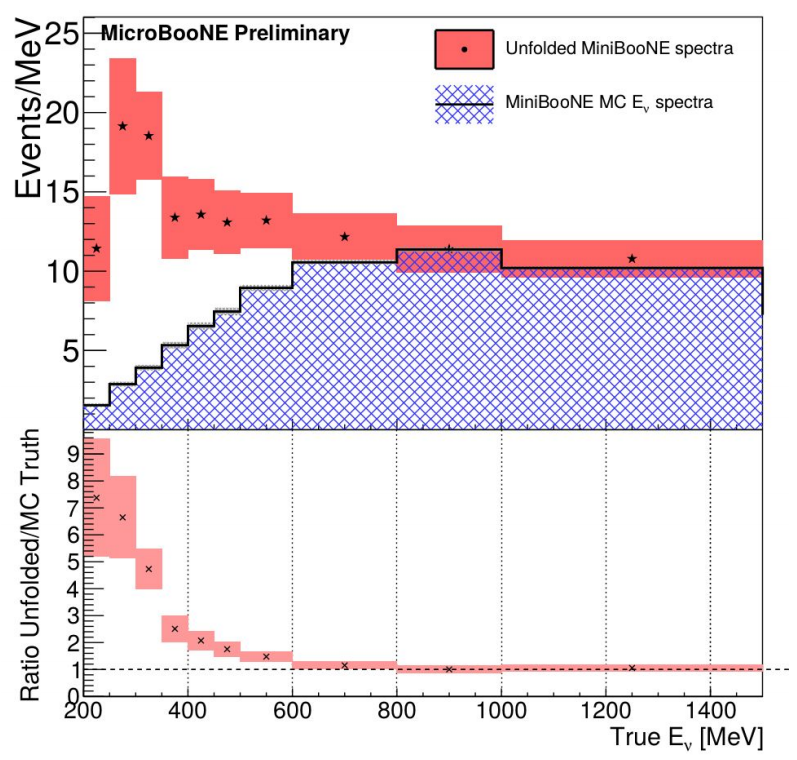
\includegraphics[width=0.45\textwidth]{Sensitivity/lee_unfolded_signal.png}
    \caption{If the intrinsic \nue flux was the red histogram instead of the predicted blue histogram then the observed excess and MC prediction for the reconstructed energy in MiniBooNE would match.}
    \label{fig:lee_unfolded_signal}
    \end{center}
\end{figure}
\end{comment}{}


The method used to estimate the sensitivity follows the standard prescription for a simple hypothesis test.
No parameter is extracted from the data at this stage: the hypothesis of background-only is tested against the \textit{simple} hypothesis of background-plus-signal, with signal being the LEE unfolded signal.
The procedure is described below:
\begin{itemize}
    \item Choice of the observables, typically one or more histograms. For this analysis, this consists in the reconstructed energy spectrum for a \nue selection plus a reconstructed energy spectrum of a \numu selection for the constraint of the systematic uncertainties. The energy reconstruction used for \nue and \numu events is defined in sec.~\ref{sec:ereco}. 
    \item Choice of the test statistic, which is a function of the observables only. This variable condenses all information of the observables in one number. Different choices are described in the following subsection. The primary result is obtained with a $\Delta\chi^2$ test-statistic using the $\chi^2_CNP$ formalism \cite{bib:Ji_2020}, as implemented in SBNFit.
    \item Definition of the two hypotheses, where $H_0$ is the null hypothesis and $H_1$ is the alternate hypothesis. The model used in the hypothesis can be used alternately depending on which model we want to test the sensitivity to. The two models tested in this analysis is the Standard Model (SM), where we do not observed any LEE signal, and the LEE model, where we do observe the LEE signal.
    \item Toy-experiments or pseudo-experiments. The expected distributions of the test statistic under the two hypotheses are built by randomly sampling the observables from their expected distributions. In case of the statistical only sensitivities, the bins of the histograms are treated as independent Poisson variables. In case systematic uncertainties are considered, the bins of the histograms are treated as a Multivariate Gaussian distribution, determined by the mean values and by a covariance matrix, which is then convoluted with a Poisson sampling that accounts for the statistical fluctuations.
    \item Once each toy-experiment is performed, and a distribution for the bin contents of the histograms is observed, the significance to rule out the $H_0$ hypothesis assuming that the $H_1$ hypothesis is true can be computed. This is done by computing the value of the test statistic associated to the observation, and then the p-value with respect to the expected distribution of the test statistic under $H_0$.
    \item To compute the expected significance, we can consider the median value, and an interval which contain 68\% (or 95\%) of the distribution of the test statistic under $H_1$, and compute the p-values with respect to $H_0$.
    \item The p-value is typically converted to the number of sigma of a standard Gaussian that produces the same p-value, as outlined in \cite{bib:cowan}.
\end{itemize}

\subsection{Statistics-Only Sensitivities }
\label{subsec:teststats}

Statistics-only sensitivities are computed using the SBNfit tool~\cite{bib:sbnfitgit}. To estimate the sensitivity of the MiniBooNE LEE unfolded signal, SBNfit uses the following $\Delta \chi^2$-like variable as the test statistic:
\begin{equation}
\label{eqn:deltachi2}
\begin{comment}
\Delta\chi^2 = \sum_{i=1}^{N}\left( \frac{(n^i - \mu^i_{H_0})^2}{\mu^i_{H_0}} - \frac{(n^i - \mu^i_{H_1})^2}{\mu^i_{H_1}} \right)
\end{comment}
\Delta\chi^2 = \sum_{i,j=1}^{N}\left( (n^i - \mu^i_{H_0})E_{i,j}^{-1}(n^j - \mu^j_{H_0}) - (n^i - \mu^i_{H_1})E_{i,j}^{-1}(n^j - \mu^j_{H_1})\right),
\end{equation}
where $i$ is the index of the bin, $n_i$ is the observed number of entries in that bin, whereas $\mu^i_{H_0, 1}$ is the expected number of entries under the null and alternative hypotheses, respectively, and $E_{i,j}$ is the statistical covariance matrix that approximates Poisson statistical errors in the matrix diagonals as follows,
\begin{equation}
    E_{CNP}^{stat} \equiv 3/\left( \frac{1}{n^i} + \frac{2}{\mu^i_{H_0}} \right) \delta_{ij}.
\end{equation}
The statistics-only sensitivity to the LEE signal with the combined \npsel and \zpsel selection is found to be $2.5\sigma$ with SBNFit, as illustrated in figure~\ref{fig:1eNp:SBNFit:statonlysensitivity}.

\begin{figure}[ht] 
\begin{center}
    \begin{subfigure}[b]{0.48\textwidth}
        \centering
        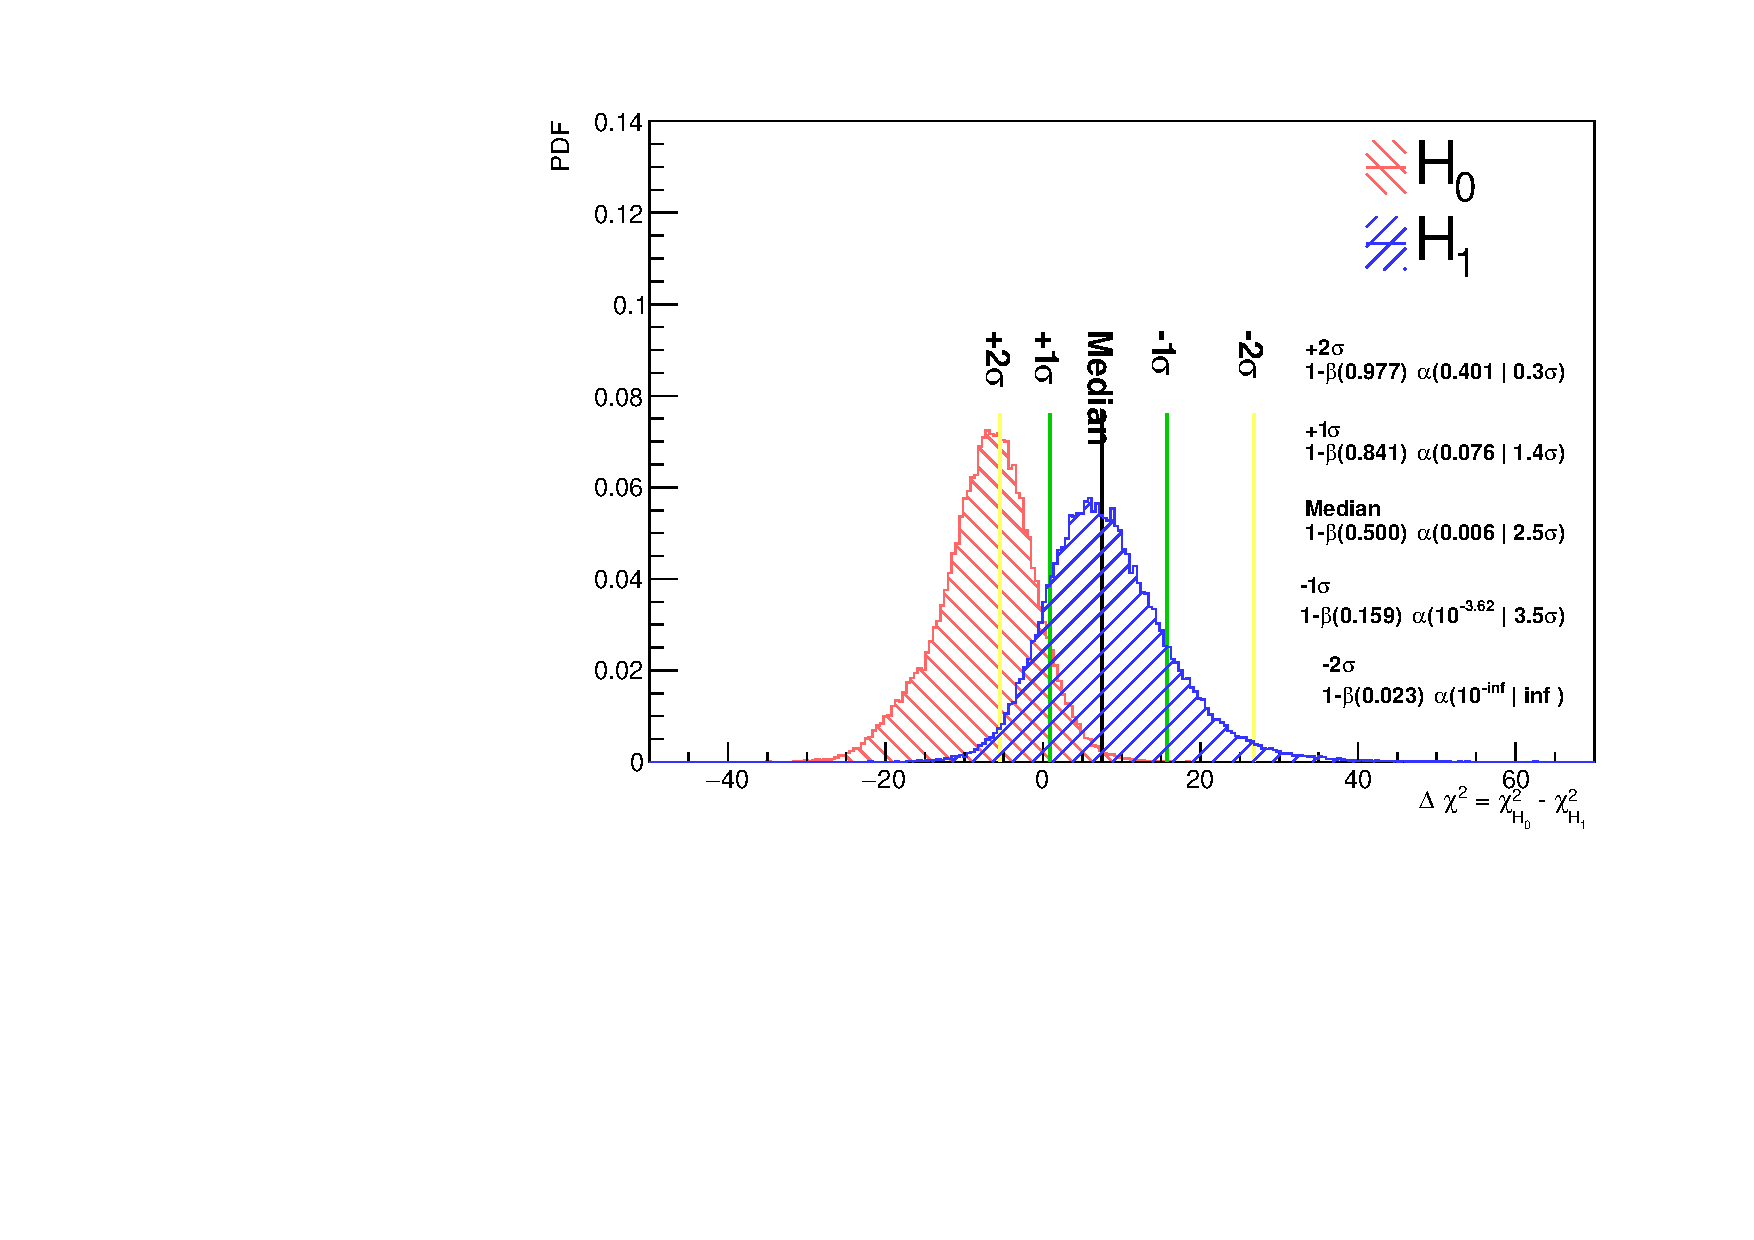
\includegraphics[width=1.\textwidth]{Sensitivity/sensitivity-run123/SBNfit_Cls_nue_1e0p_reco_e_H1_mc_collab_statsonlyCNP_Chi.pdf}
        \caption{ruling out SM if LEE is true}
    \end{subfigure}
        \begin{subfigure}[b]{0.48\textwidth}
        \centering
        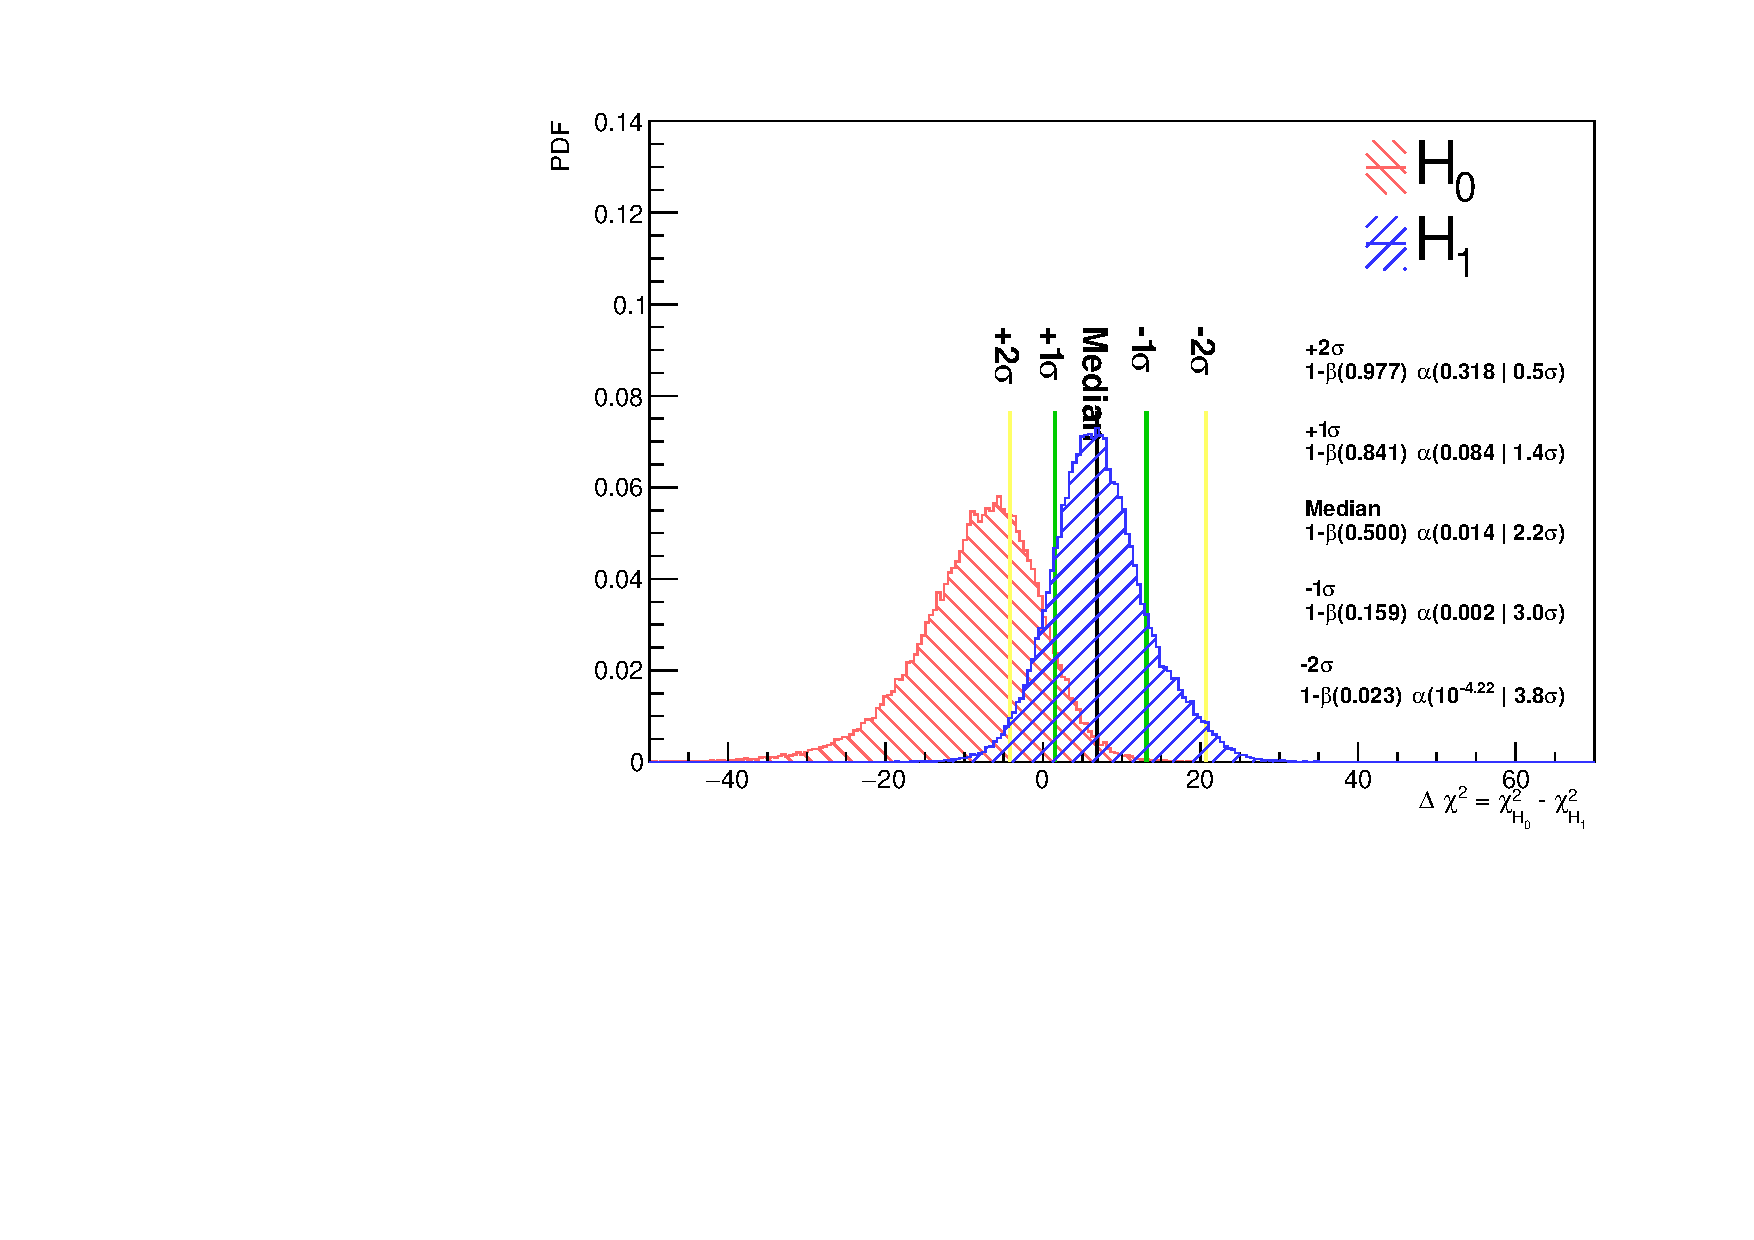
\includegraphics[width=1.\textwidth]{Sensitivity/sensitivity-run123/SBNfit_Cls_nue_1e0p_reco_e_H1_mc_collab_statsonly_exclusionCNP_Chi.pdf}
        \caption{ruling out LEE if SM is true}
    \end{subfigure}
\caption{Distribution of the test statistics under the null and alternative hypotheses for statistical-only sensitivities studies. This study use the combined samples of run 1, run 2, and run 3 scaled to $6.95\times10^{20}$ POT. (a) $H_0$ is the standard model and $H_1$ is the LEE model, (b) $H_0$ is the LEE model and $H_1$ is the standard model.}
\label{fig:1eNp:SBNFit:statonlysensitivity}
\end{center}
\end{figure}

\begin{comment}
\subsubsection{Treatment of Statistical Errors in SBNFit}
\label{sec:systematics:stat}
\par In the SBNFit version used to produce this note, statistical uncertainties for the computation of the $\chi^2$ used for the sensitivity estimation are taken as $\sqrt{N}$ with $N$ the number of entries in a bin. In computing the sensitivity, Poisson statistics are used to generate toy MC datasets. For bins with zero expected background events from the off-beam EXT sample, a statistical uncertainty on this number is computed by taking the mean of the Poisson distribution that gives a value of 0 in 68\% of draws. We use the value of 0.4 (${\rm Poisson}(0,\mu=0.4) = 0.670$). This number is then scaled by the weight applied to EXT data ($\sim0.8$). This leads to including a diagonal absolute uncertainty in the covariance matrix of 0.32 for bins with no EXT contribution, which therefore allows for EXT contributions in each bin in the drawing of toy experiments. Future iterations of the sensitivity will update the $\sqrt{N}$ treatment of statistical uncertainties in the covariance matrix used to calculate the $\chi^2$ test-statistic, as illustrated in DocDB 29239~\cite{bib:statMike}.
\end{comment}

\subsection{Sensitivities with systematic uncertainties }
\label{subsec:sensitivity_syst_uncertainty}
%Two different studies have been performed to estimate the sensitivity in presence of systematic uncertainties.

Accounting for systematics in the SBNFit framework involves two modification to the previous analysis: modifying the $\Delta \chi^2$ test statistic, and sampling according to the systematic uncertainties.
The effect of the systematic uncertainties on the observables can be condensed in the covariance matrix, which is obtained by marginalising over the systematic uncertainties, as seen in \ref{sec:systematics}.

The $\Delta \chi^2$ is modified as follows taking into account the covariance matrix which includes both statistical and systematic uncertainties on the null hypothesis only. The $\chi^2_{CNP}$ formalism is also used in the $\chi^2$ test-statistics and can be written as follows.
\begin{equation}
\label{eqn:deltachi2_systematic}
\Delta\chi^2 = \sum_{i,j=1}^{N}\left( (n^i - \mu^i_{H_0})E_{i,j}^{-1}(n^j - \mu^j_{H_0}) - (n^i - \mu^i_{H_1})E_{i,j}^{-1}(n^j - \mu^j_{H_1})\right) ,
\end{equation}
where covariance matrix can be written as 
\begin{equation}
E_{ij} = E_{CNP}^{stat} + E_{ij}^{syst}.
\end{equation}
This second test statistic is more optimal in the case systematic uncertainties are present.

Secondly, SBNfit uses the covariance matrix to properly sample from the covariance matrix.
The toy experiments can be generated once the full covariance matrix is in hand. Assuming that the covariance matrix is a symmetric, positive-definite matrix, the procedure to generate these toy experiments is as follows:
\begin{enumerate}
    \item A Cholesky decomposition \cite{bib:cholesky} is performed on the covariance matrix: $$E = LL^{T},$$
    where $L$ is a lower triangular matrix.
    \item A vector $v$ with length equal to the number of bins as the selection is generated, where each of the $i$ elements of $v$ are drawn from a Gaussian distribution with mean zero and standard deviation equal to one.
    \item A Poisson fluctuated toy data histogram is given by
$$x_{toy} = x_{CV} + Lv.$$
    % \item We follow the same procedure to test the LEE hypothesis as described in the Section~\ref{subsec:teststats}
\end{enumerate}

% Nico: added in the previous subsection
% \begin{figure}[H]
% \begin{center}
% 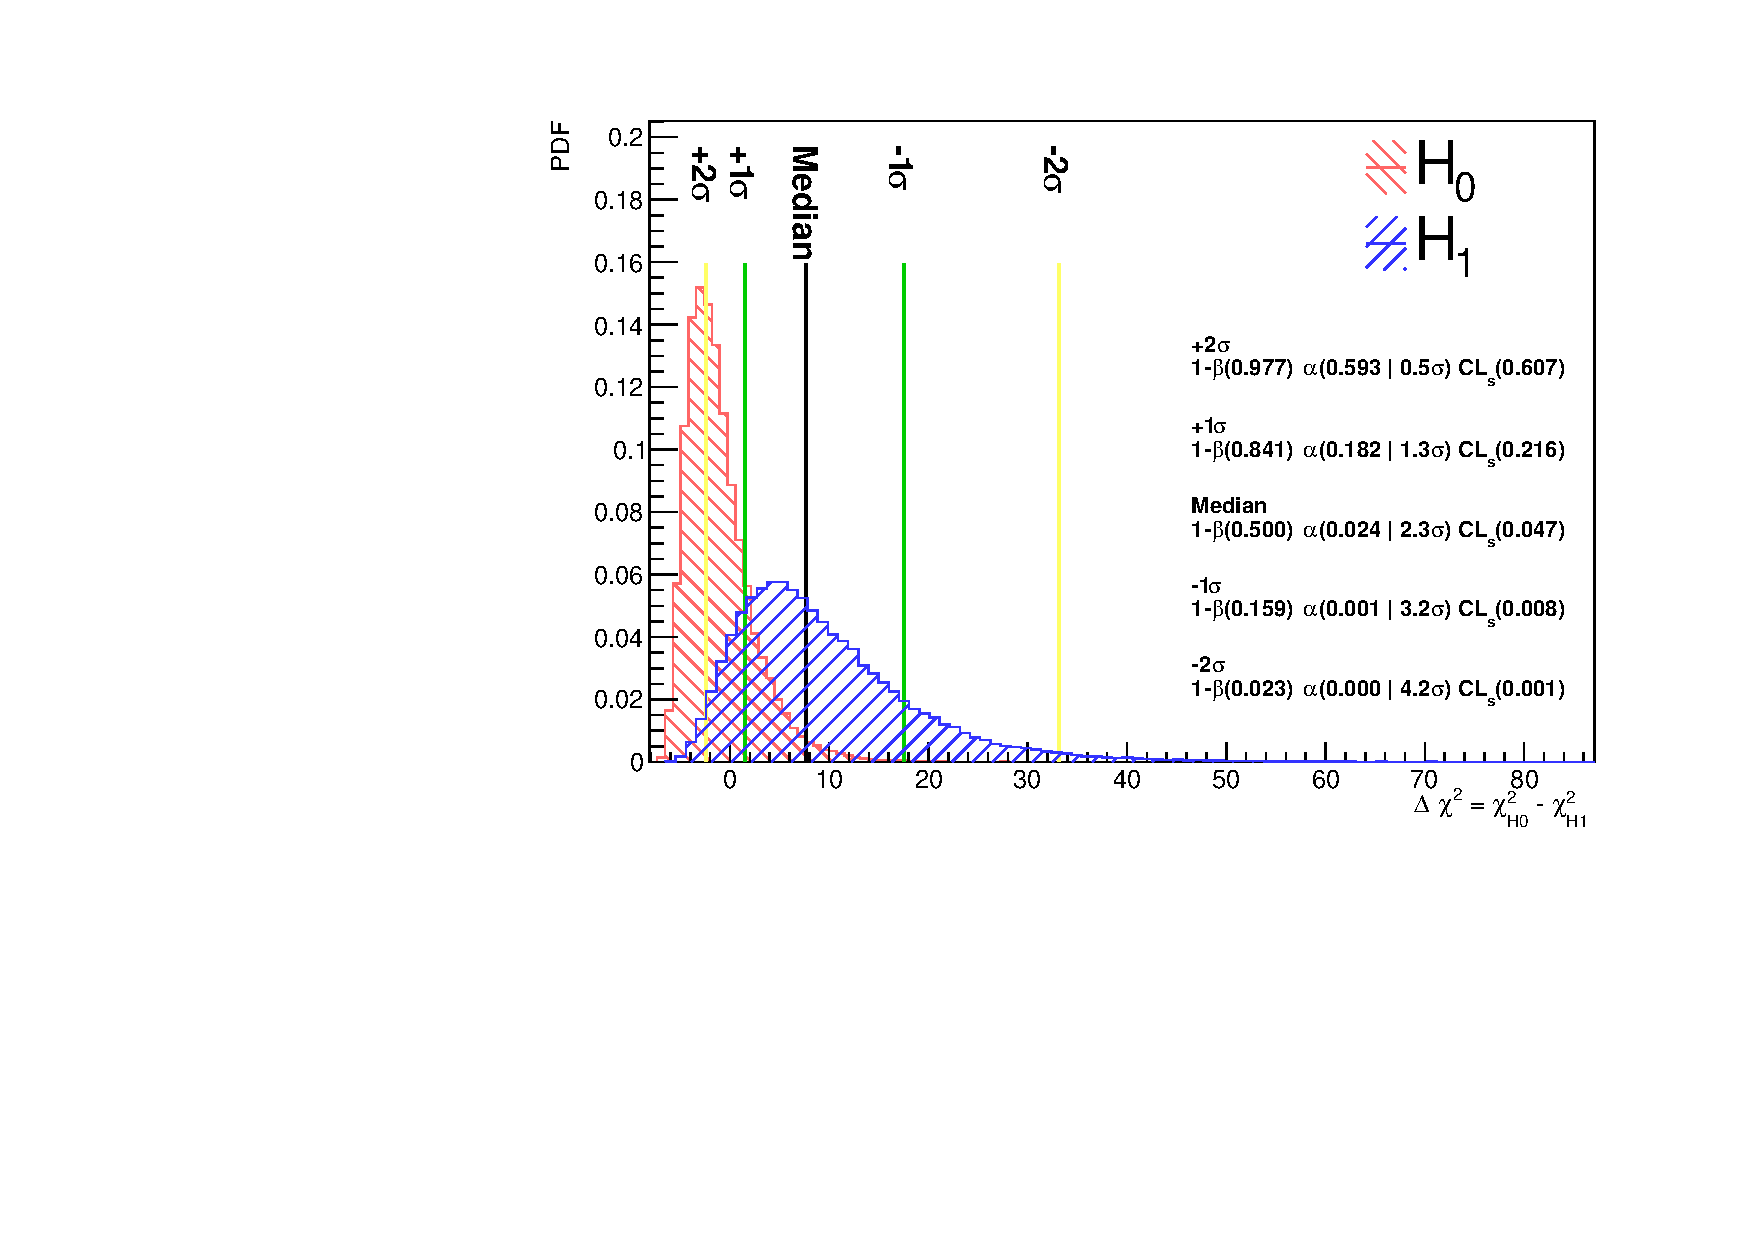
\includegraphics[width=0.45\textwidth]{Sensitivity/SBNfit_Cls_nue_reco_e_genietune_run1_LEE_deltachi_statonly.pdf}
% \caption{\label{fig:1eNp:box:statonlysensitivity} Statistics-only sensitivity estimation for the 1eNp box cut selection. Sample is taken from Monte Carlo Run 1 Data and scaled to $1.01\times10^{21}$ POT}
% \end{center}
% \end{figure}
The resulting plot of the test statistic described in eq. \ref{eqn:deltachi2_systematic}, and utilizing systematics as presented in ~\cref{tab:1eNp0pi_bdt_errors} and ~\cref{tab:1e0p0pi_bdt_errors} before applying any constraint, is shown in figure \ref{fig:1eNp:BDT:statsystsensitivityrun1to3}. 
The median sensitivity obtained including flux, cross-section, hadron reinteractions, and detector systematic uncertainties is $2.3\sigma$ from the combined fit of the \npsel and \zpsel selections, with no \numu constraint.
%This calculation is performed without sideband constraints.

\begin{figure}[H]
    \centering
    \begin{subfigure}[b]{0.48\textwidth}
    \centering
    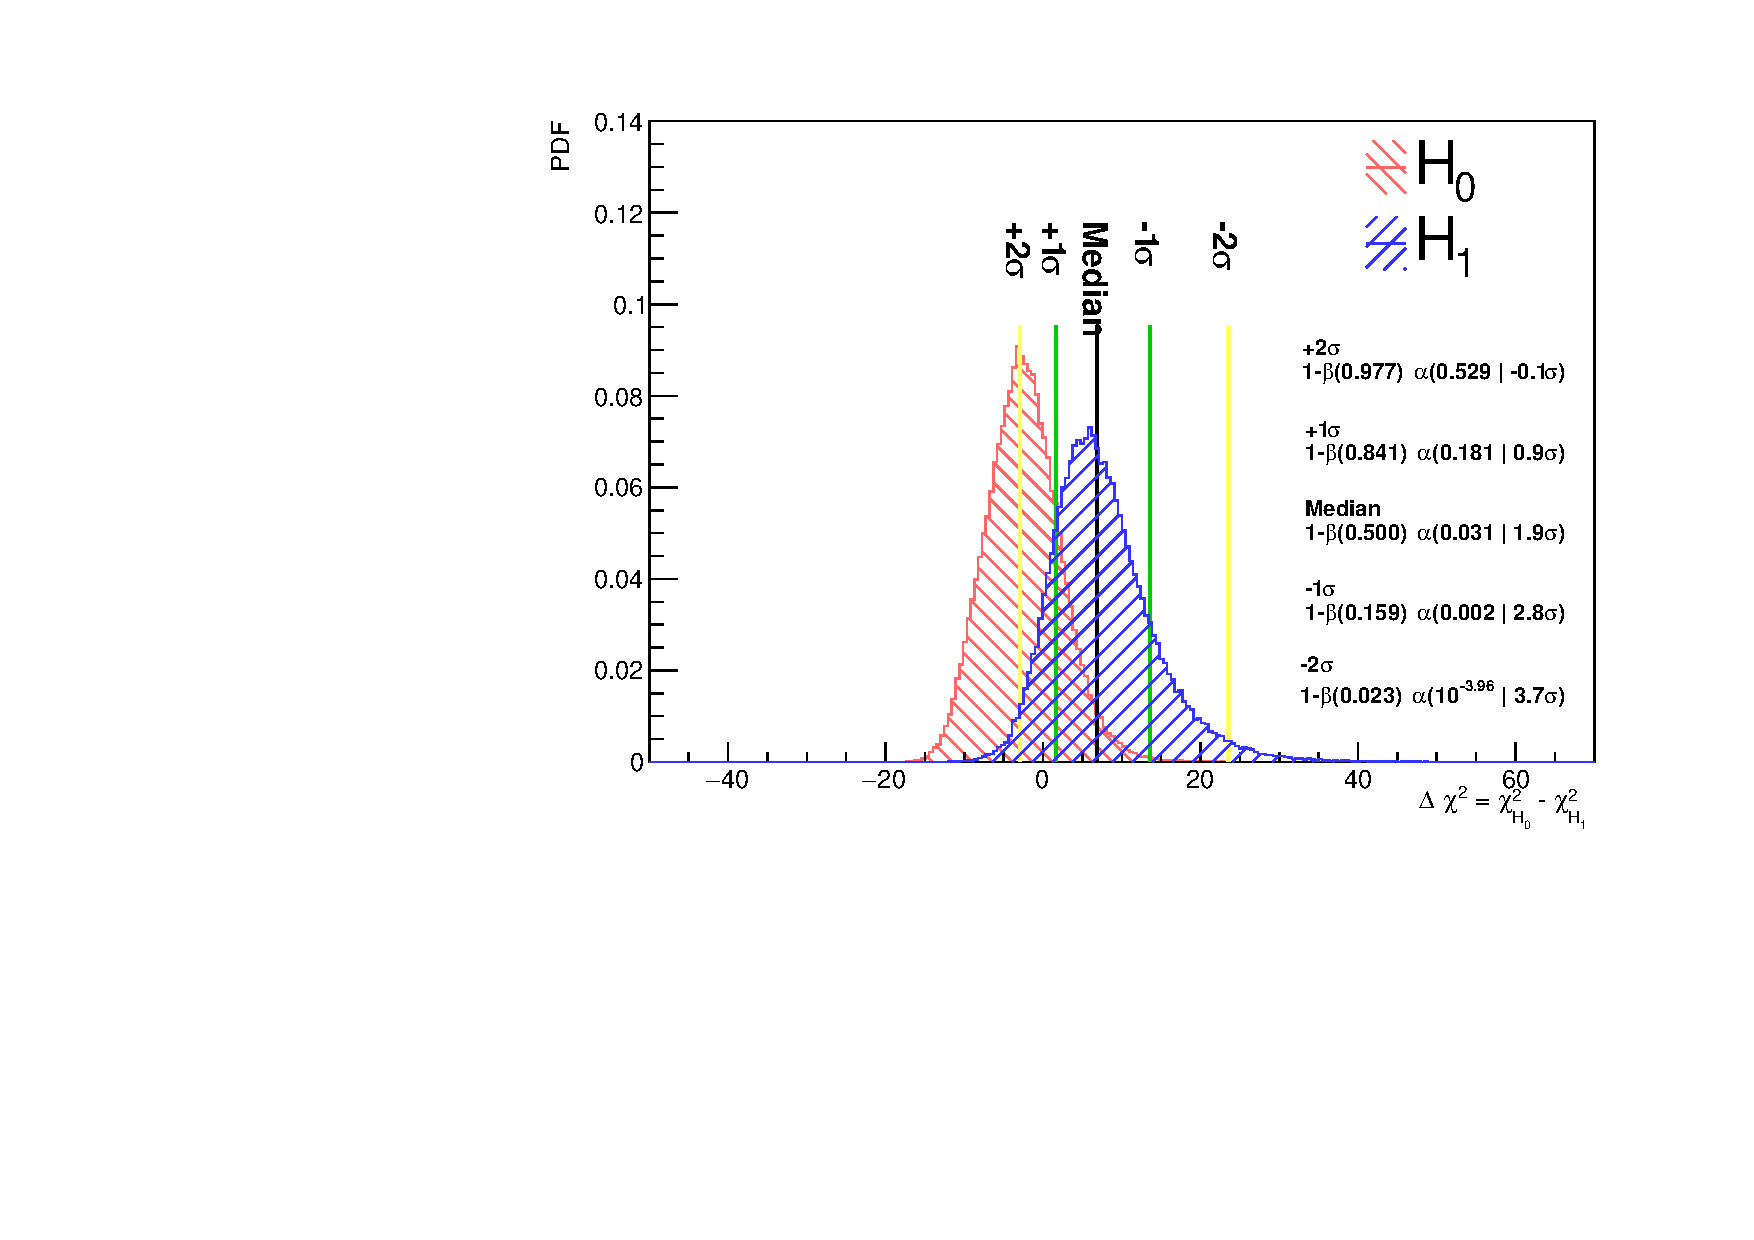
\includegraphics[width=1.00\textwidth]{Sensitivity/sensitivity-run123/SBNfit_Cls_nue_1e0p_reco_e_H1_mc_collab_syst_detsysCNP_Chi.pdf}
    \caption{ruling out SM if LEE is true}
    \end{subfigure}
    \begin{subfigure}[b]{0.48\textwidth}
    \centering
    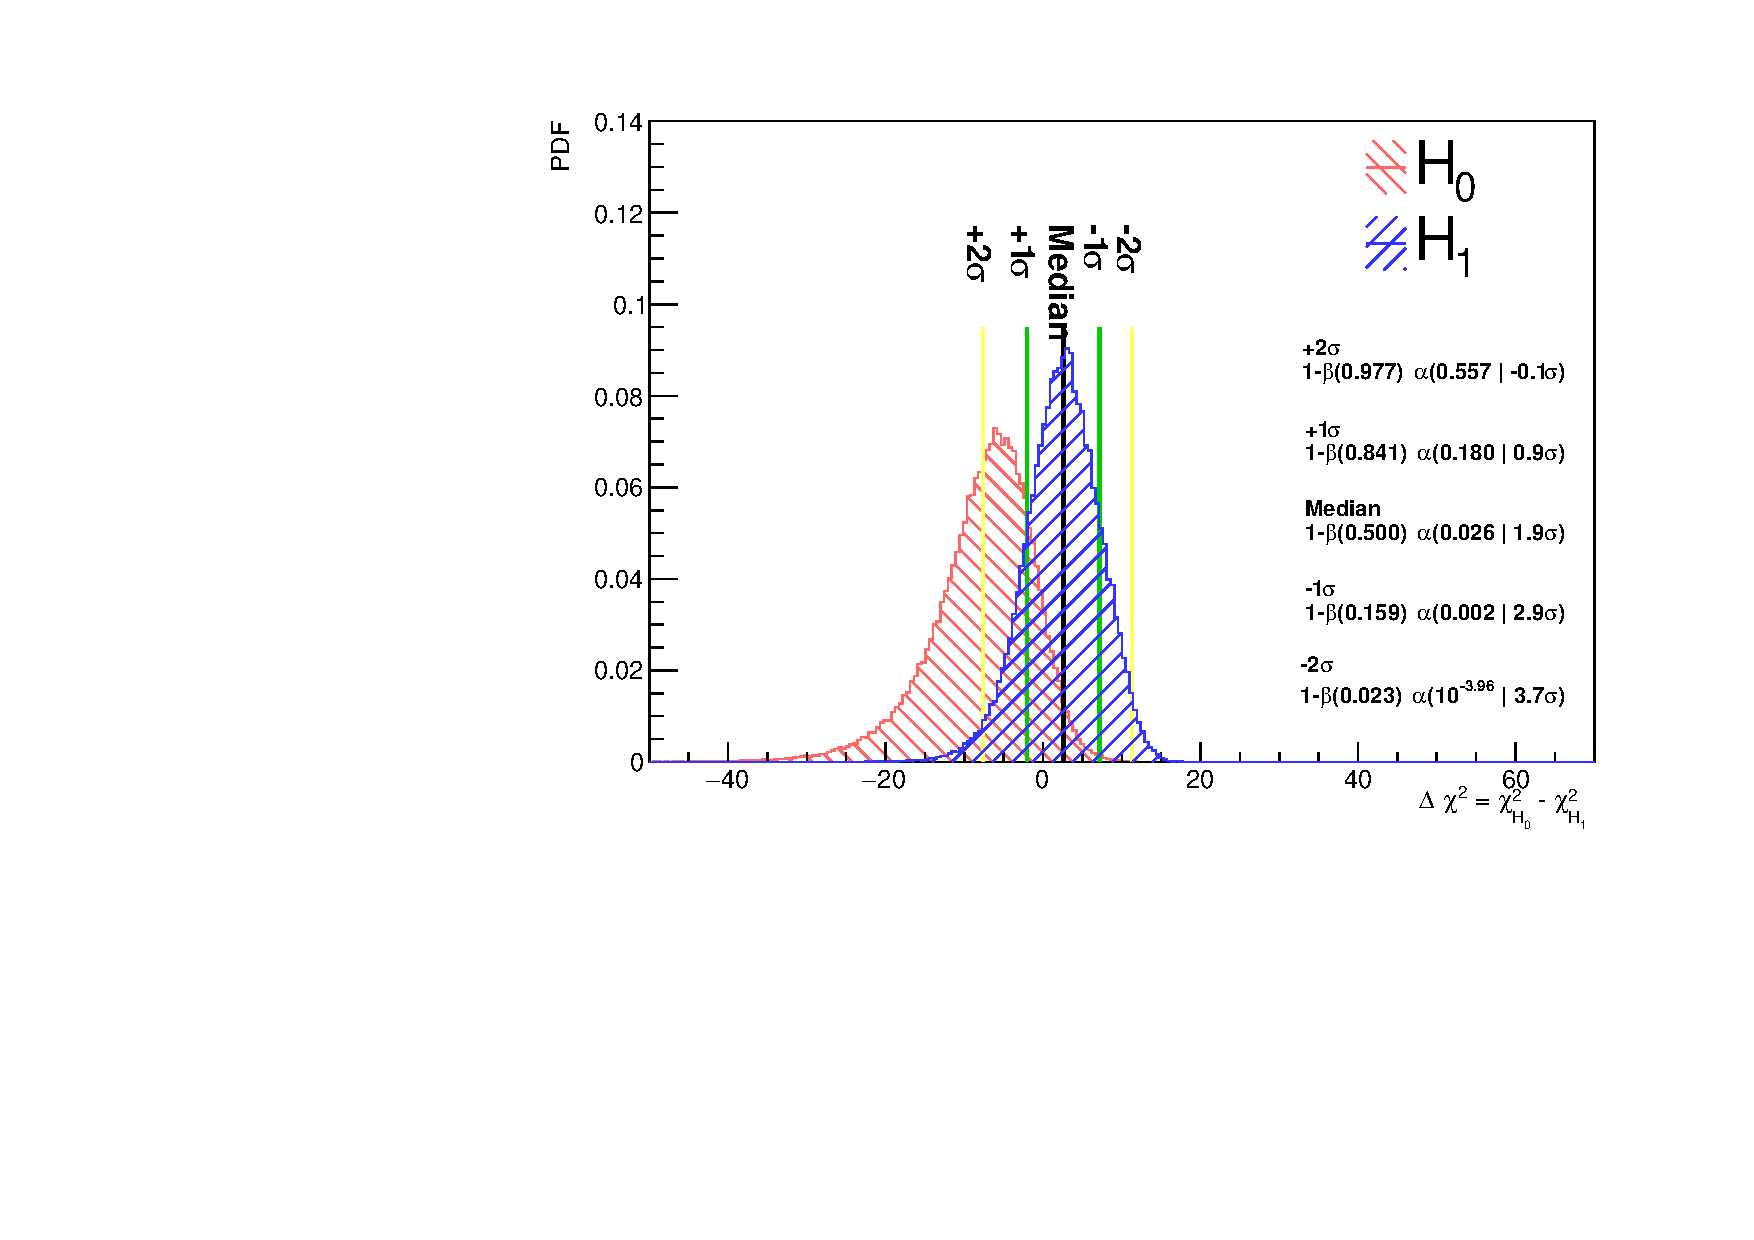
\includegraphics[width=1.00\textwidth]{Sensitivity/sensitivity-run123/SBNfit_Cls_nue_1e0p_reco_e_H1_mc_collab_syst_detsys_exclusionCNP_Chi.pdf}
    \caption{ruling out LEE if SM is true}
    \end{subfigure}
    \caption{Statistics and Systematics (cross-section, flux, g4, and detector systematics) sensitivity estimation for the \npsel and \zpsel selection without the \numu constraint. Sample is taken from combined Monte Carlo samples of Run 1, Run 2, and Run 3 and scaled to $6.95\times10^20$ POT.  (a) $H_0$ is the standard model and $H_1$ is the LEE model, (b) $H_0$ is the LEE model and $H_1$ is the standard model.}
    \label{fig:1eNp:BDT:statsystsensitivityrun1to3}
\end{figure}

%A second and simpler exercise is performed to get a rough understanding of the degradation of the sensitivity due to the presence of systematic uncertainties, using Nicol\`o's tool.
%The sampling of toy-experiments is performed by adding, in addition to the statistical bin content fluctuations, a Gaussian sampling independent for each bin with mean equal to the expected value of the bin content and standard deviation set to a fixed fraction of uncertainty. We choose a value of 20\%: the average level of systematic uncertainty seen in the MCC8 \numucc inclusive analysis~\cite{bib:numuCCincl}.
%This process is equivalent to sample from a diagonal covariance matrix, with fractional uncertainties is set to the desired value.
%Results from this method are shown in figure \ref{fig:sensitivity_function_pot}.

\subsection{How Constraints and Systematics are included in the 1$e$N$p$ Sensitivity Calculation }
\label{ssec:finalSensitivityCalc}

The multiple selections described in  chapters~\ref{sec:nueselection} and~\ref{sec:numuselection} share the same neutrino flux and cross-section model, and therefore the measurements between them are highly correlated. 
We can exploit these correlations to reduce the systematic uncertainties when performing the combined side-by-side fit of the different channel for the sensitivity results. 
It is important to point out that the constraint procedure currently applied requires that the $\nu_{\mu} - \nu_e$ correlations exploited, and more generally the correlations between the $\nu_e$ channel and any other sideband, are representative of the underlying true correlations between these different event categories. 
A mis-modeling of these correlations can lead to an incorrect estimation of the expected $\nu_e$ rate and its uncertainties. 
Ensuring that such correlations are modeled correctly is not a simple task. 
At a minimum, it requires a robust validation of MicroBooNE's simulation through a detailed studies of data-simulation comparisons in a broad range of variables and phase space. 

%The analysis, as presented, performs the sideband channel constraint and the final updated sensitivity calculation in two steps. This section aims to demonstrate the best estimate of the constraint that can be achieved using the selection. The analysis, in its final form, will utilize the correlation elements of the covariance matrix between the \numu and \nue events. This correlation provides the direct constraint when one forms a $\chi^2$ for the MiniBooNE's unfolded LEE signal and the \nue intrinsic which is minimized in a simultaneous combined fit. 
 
The constraint can be described as follows. Given a measurement of events in a defined sideband (the \numu in this case), the $\nu_e$ prediction and uncertainties on their prediction are updated informed by the observed data. This is achieved thanks to the inclusion, in the $\chi^2$ expression, of the observed data-MC differences in the \numu channel, which help constrain modeling uncertainties and carry those constrained uncertainties to the \nue measurement through the constructed correlations.
This has the effect of reducing systematic uncertainties provided the observed data is compatible with the original predicted event rates within systematic uncertainties. As a second step, the updated (reduced) systematic uncertainties (which take the form of a new covariance matrix $E_{ij}$ as defined in eq.~\ref{eqn:deltachi2_systematic}) are used to compute the sensitivity post-constraint following the same procedure outlined in sec.~\ref{subsec:sensitivity_syst_uncertainty}. This two-step procedure was used to cross-check the robustness of the constraint procedure and its effects on improving the sensitivity of the \npsel selection. The results of this can be seen in \cref{app:sensitivity}.
%while not a simultaneous combined fit of the $\nu_{\mu}$ and $\nu_e$ channels, is in practical terms equivalent in the regime where the number of events in the \nue channel is much smaller than those in the \numu sideband~\footnote{Nonetheless, advantages to the simultaneous combined fit exist, as described in slide 10 of \href{https://microboone-docdb.fnal.gov/cgi-bin/private/RetrieveFile?docid=7635&filename=Constraining\%20Nue\%20Uncertainties.pdf&version=1}{DocDB 7635}}.

The technical method used to constrain systematic uncertainties through a sideband with the covariance matrix formalism is illustrated in Sec. 1 of MiniBooNE TN 221, available on \href{https://microboone-docdb.fnal.gov/cgi-bin/private/RetrieveFile?docid=7583&filename=Constraining\%20the\%20nue\%20Background\%20Uncertainties\%20with\%20the\%20Observed\%20\%20numu\%20\%20Events\%20tn221.pdf&version=1}{DocDB 7583}. The constraint procedure is performed by constructing a covariance matrix, $E_{ij}$, of combined \npsel and $\nu_\mu$ channels as well as \zpsel and $\nu_\mu$ channels. The systematics constraint is provided by the correlation elements between the events in the \npsel, \zpsel and $\nu_\mu$ selection when we minimize the $\chi^2$ between the data and MC in these selection. 

In this procedure, to constrain the uncertainties in the \npsel or \zpsel channel, we assume that the observed events in the \numu ($N_{\rm data}$) are equal to the predicted events ($N_{MC}$) within the statistical errors. The covariance matrix is updated by adding the statistical error of the \zpsel and $\nu_\mu$ channels, respectively, to the diagonal of the inverted covariance matrix as follows:
\begin{equation}
    (E_{ij}^{-1})^{(new)} = E_{ij}^{-1} + \frac{1}{N_{MC}} 
\end{equation}
The new matrix, $(E_{ij}^{-1})^{(new)}$, is then inverted to give the constrained covariance matrix, $(E_{ij})^{new}$.
Several closure-tests of this procedure have been performed as part of the validation of this analysis. They are presented in appendix~\ref{app:closure}. 
%The \zpsel selection is currently only exercised to constraint the systematics of the \npsel channel. However, for the final analysis, the \zpsel channel is going to be included as part of the $\nu_e$ signal channel fit of the sensitivity calculation. 

%The different selections described in Section~\ref{sec:nueselection} provide constraints to different energy range of the 1eNp selection as well as the kinematics and topology. The inclusive $\nu_e$ selection can be used to constrain the high energy $\nu_e$. We explore the prospect of adding the inclusive $\nu_e$ selection to constrain the high energy $\nu_e$. Given the non-orthogonality of this selection to the 1eNp0$\pi$ selection, we still need to explore other variables that can provide orthogonality in order to exercise the constraint. The 1e0p0$\pi$ channel can provide constraint to the less understood proton reconstruction and kinematics. The CC and NC $\pi0$ samples can be utilized to constrain the uncertainties coming from shower. Finally, we can use the $\nu_\mu$ selection to constrain the flux and cross section at low energy $\nu_e$ and Section~\ref{subsec:constraintfromnumu} describes this in more details. In its current state, the analysis utilizes the combined $\nu_{\mu}$ and \zpsel channel as constraints for $\nu_e$ systematics. Constraints employing the $\pi^0$ channels will be implemented in future iterations of this work.

%\subsubsection{Constraint from $\nu_\mu$ and \zpsel Selections}
\subsubsection{Constraint from $\nu_\mu$ selections on the \npsel selection}
\label{subsec:constraintfromnumu}

Using the measured $\nu_{\mu}$ channel to constrain $\nu_e$ systematics is an approach used in several accelerator-based neutrino oscillation experiments. In particular, this was performed in the \nue analysis in MiniBooNE. This constraint takes advantage of the high statistics $\nu_{\mu}$ data and modeled correlations between electron and muon neutrino flux, cross sections, and hadron reinteractions. %We also leverage the multiple selections within this analysis to provide additional constraint to the \npsel selection by utilizing the \zpsel channel. The \zpsel channel provides a valuable constraint for the less understood proton reconstruction and kinematics when we perform the simultaneous combined fit, which is not going to be demonstrated in this section.
The constraint demonstrated in this section is exercised through the covariance matrix constructed in the energy spectrum of $\nu_e$, and $\nu_{\mu}$. 
Figure~\ref{fig:bdt_corr_matrix} displays the correlation matrix between \npsel $\nu_e$, \zpsel $\nu_e$, and $\nu_{\mu}$ channels for the BDT \nue selections (a similar matrix for the Box-Cuts is found in fig.~\ref{fig:boxcut_corr_matrix}). The correlation between the elements in the matrix allow to constrain $\nu_e$ uncertainties through the measurements of correlated $\nu_{\mu}$ events. 
The non-diagonal elements of the matrix represent the correlation of the flux, genie, and geant-4 systematics between the  channels. In this analysis, the detector modeling systematics are treated as uncorrelated and increase the magnitude of the diagonal elements. This has the effect of degrading the power of the correlation between the constraint channels and the \npsel channel.
%This constraint comes from the minimization of the $\chi^2$ when we fit both the 1eNp $\nu_e$ and the inclusive $\nu_{\mu}$ selection to the MiniBooNE unfolded LEE signal. 
%Figure~\cite{fig:numuconstrainttruth} displays the truth-level cross section (genie) and flux correlation matrix between the two channels. 

\begin{comment}
\textit{Note that work on getting the numu constraint channel with the new genie tuned CV is still underway. 
The matrices are shown here to demonstrate the effect of the constraint which will be updated once the new $\nu_{\mu}$ constraint channel is available. 
At the time of the plots creation, the CCQE-related knobs are not included in the systematics, hence the cross section uncertainties are mostly dominated by the resonance uncertainties. 
Therefore, we observed less correlation between the $\nu_e$ and the $\nu_{\mu}$ channels at low $\nu_e$ energy.}
\end{comment}{}

\begin{figure}[ht] 
\begin{center}
    \begin{subfigure}[b]{0.45\textwidth}
    \centering
    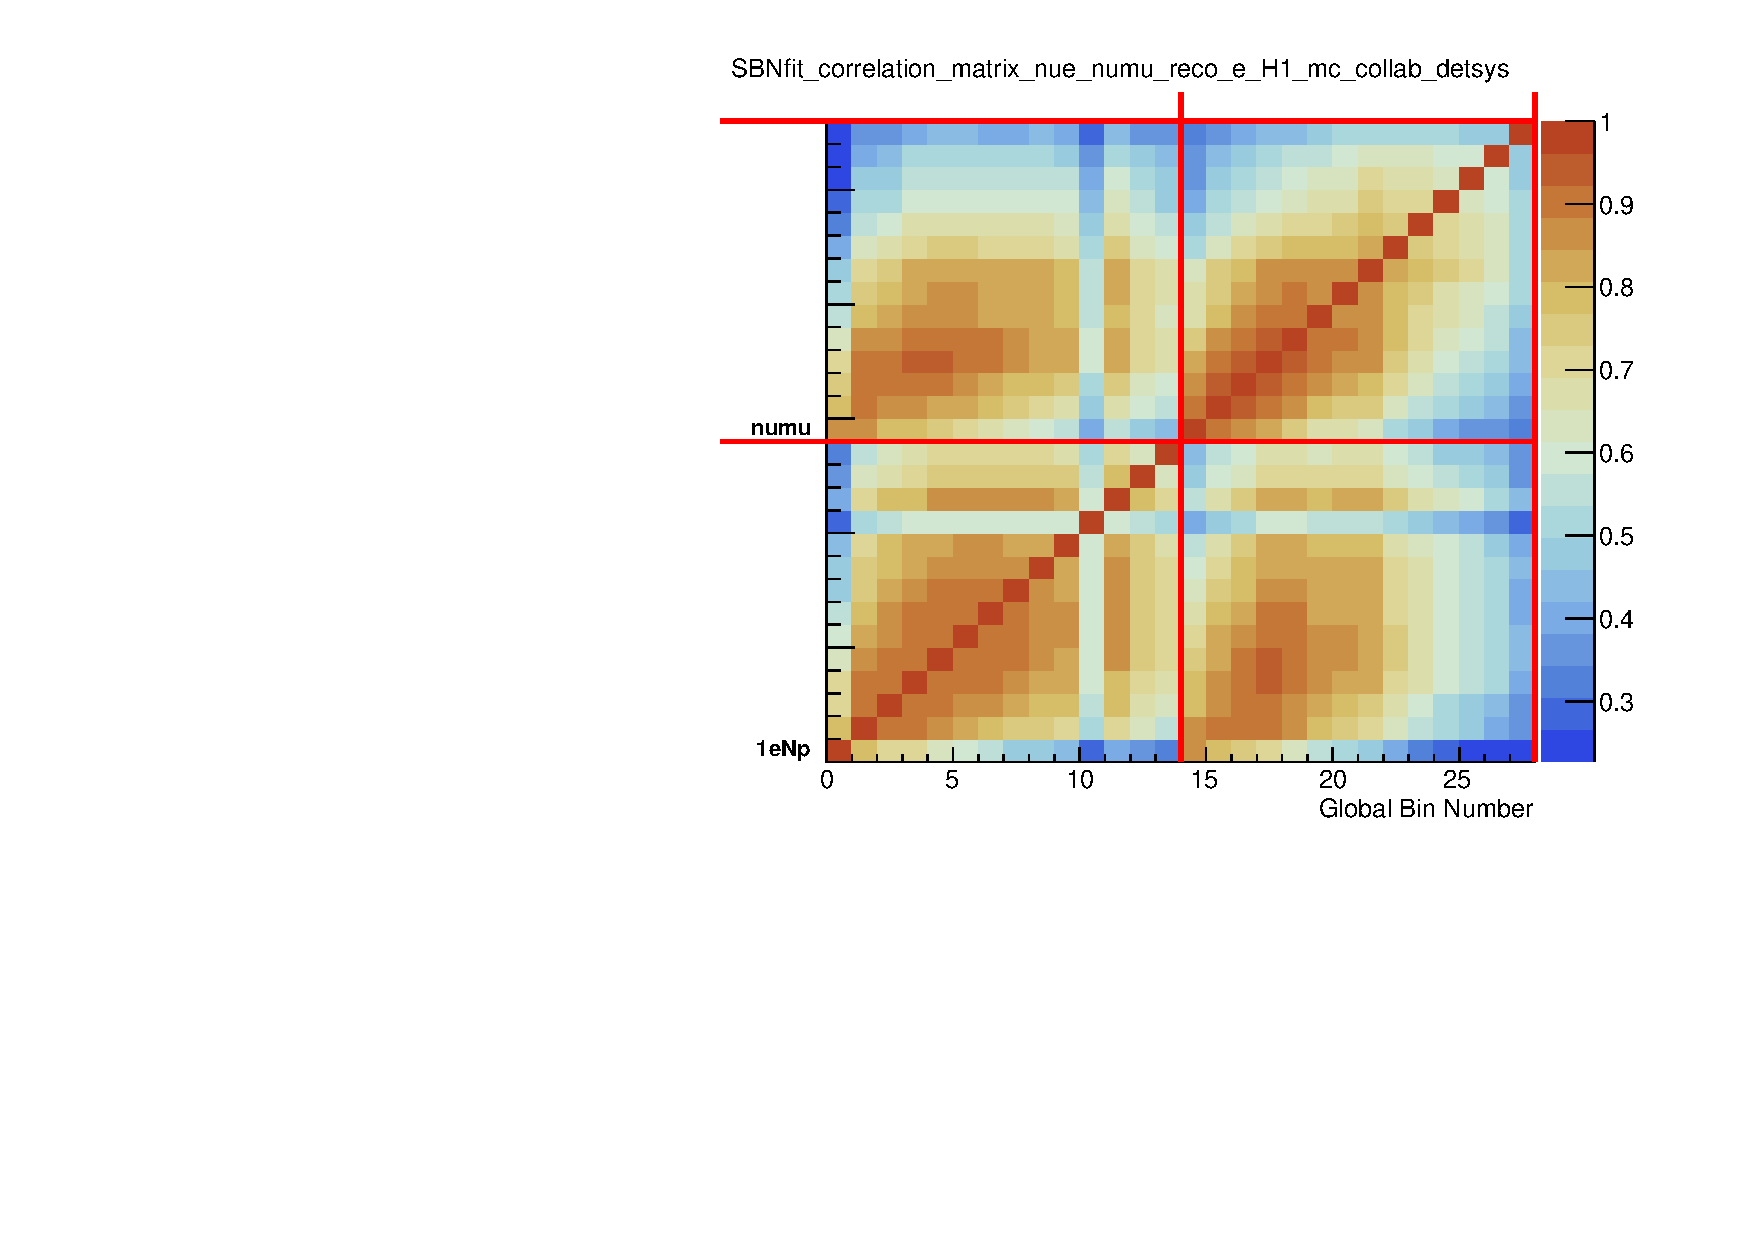
\includegraphics[width=1.00\textwidth]{Sensitivity/CorrelationMatrices/SBNfit_correlation_matrix_nue_numu_reco_e_H1_mc_collab_detsys_collapsed.pdf}
    \caption{correlation matrix for the \npsel and \numu channel}
    \end{subfigure}
    \begin{subfigure}[b]{0.45\textwidth}
    \centering
    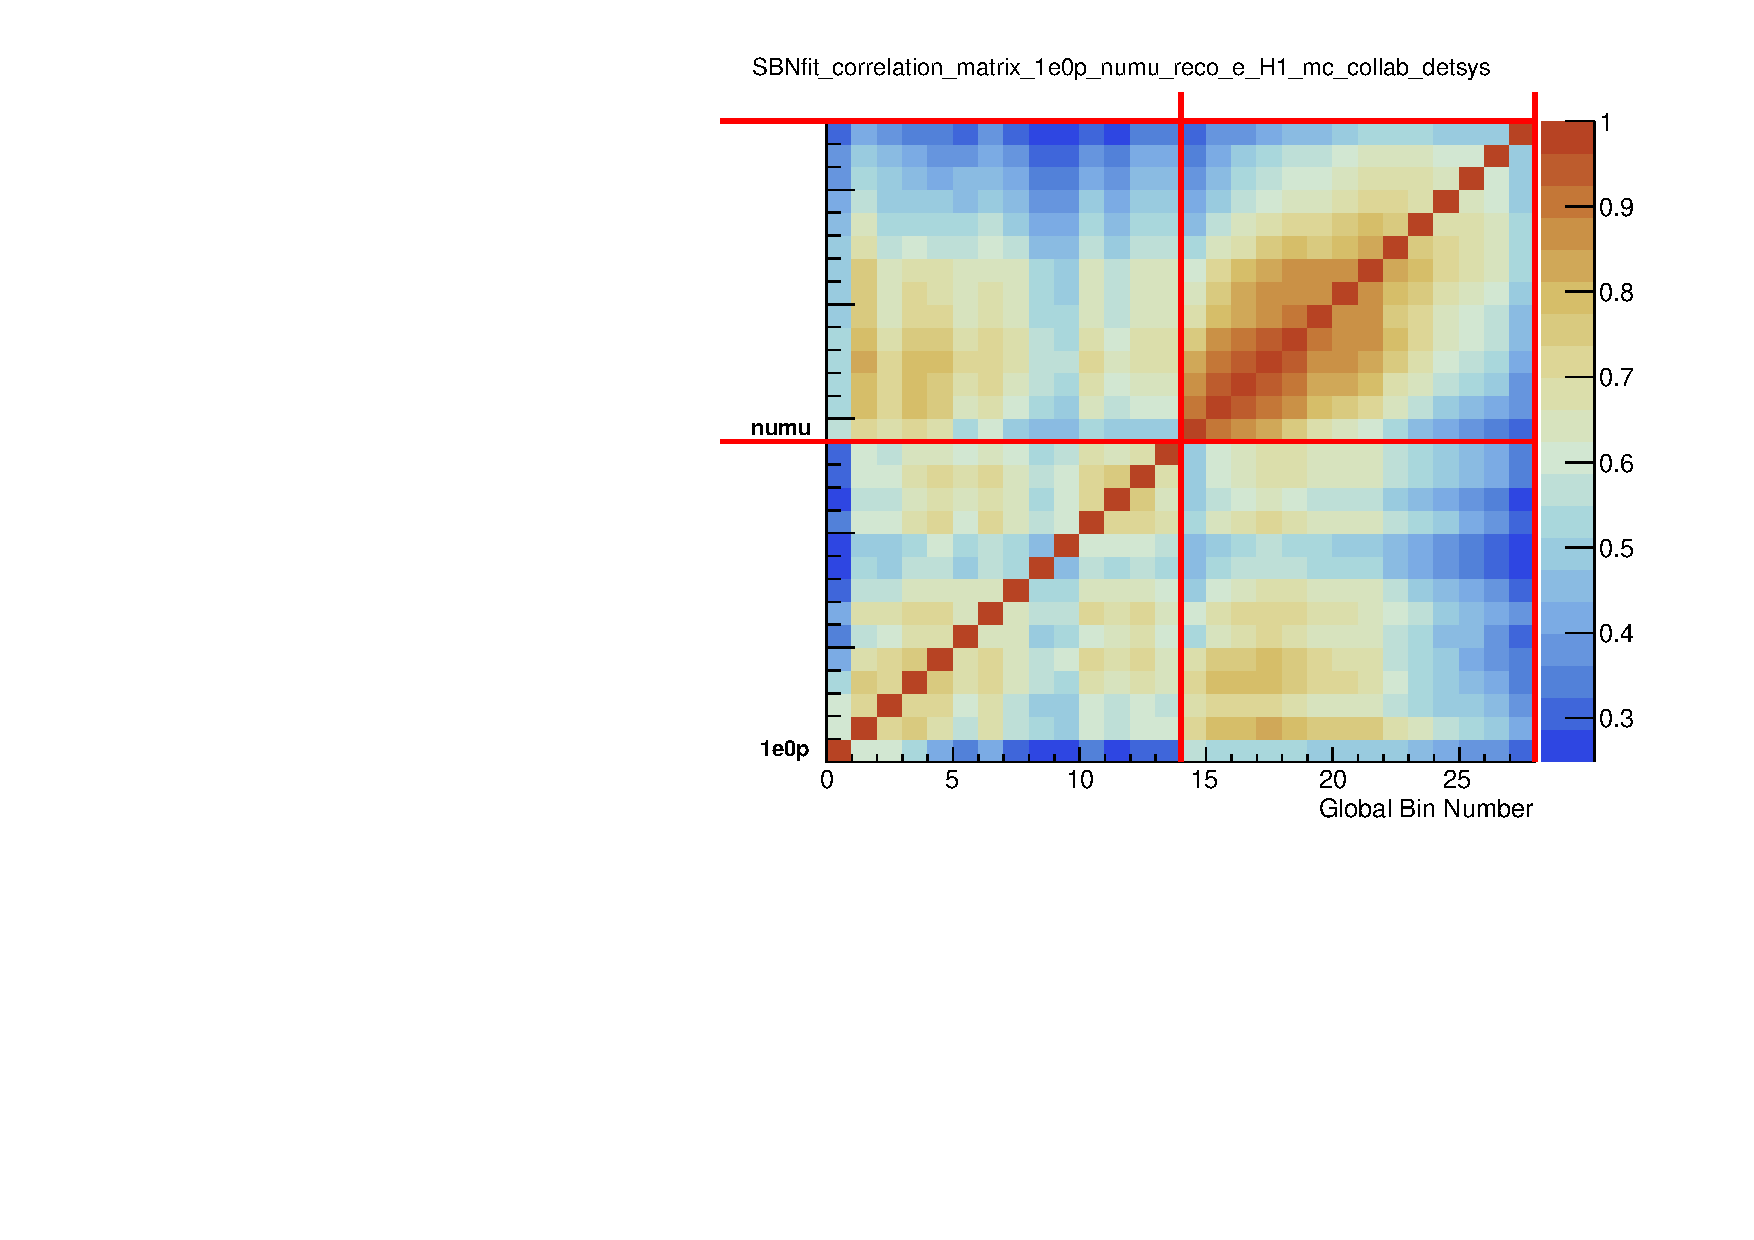
\includegraphics[width=1.00\textwidth]{Sensitivity/CorrelationMatrices/SBNfit_correlation_matrix_1e0p_numu_reco_e_H1_mc_collab_detsys_collapsed.pdf}
    \caption{correlation matrix for the \zpsel and \numu channel}
    \end{subfigure}
\caption{\label{fig:bdt_corr_matrix} correlation matrices between the \npsel, \zpsel and \numu channel, labeled accordingly on the plot.}
\end{center}
\end{figure}

\par We follow the procedures described in Document~\cite{bib:muonconstraint} to include the %\zpsel and 
\numu constraint to the covariance matrix. We make an assumption that the $N_{MC}$ is approximately the same as the $N_{signal}$ for the constraint channel. The constraint technique leads to, in this exercise, a reduction in systematic uncertainties of $\sim70$\% if we are only folding in the correlated flux, genie, and geant-4 systematics, and $\sim60$\% when we include the uncorrelated detector systematics.
Figure~\ref{fig:numuconstraintzpselnpsel} shows the effects of the $\nu_\mu$ constraint on the systematics of the \npsel $\nu_e$ selections.
% (described in sec.~\ref{sssec:NuMUCCsel:constr:muonsel} and sec.~\ref{sec:nueselection:1e0p}). %\emph{This study, is performed with the samples and muon selection developed in December 2019. This exercise will be completed with the updated central-value simulation, modeling of systematic uncertainties, and updated muon selection

\begin{comment}
\begin{figure}[ht] 
\begin{center}
    \begin{subfigure}[b]{0.45\textwidth}
    \centering
    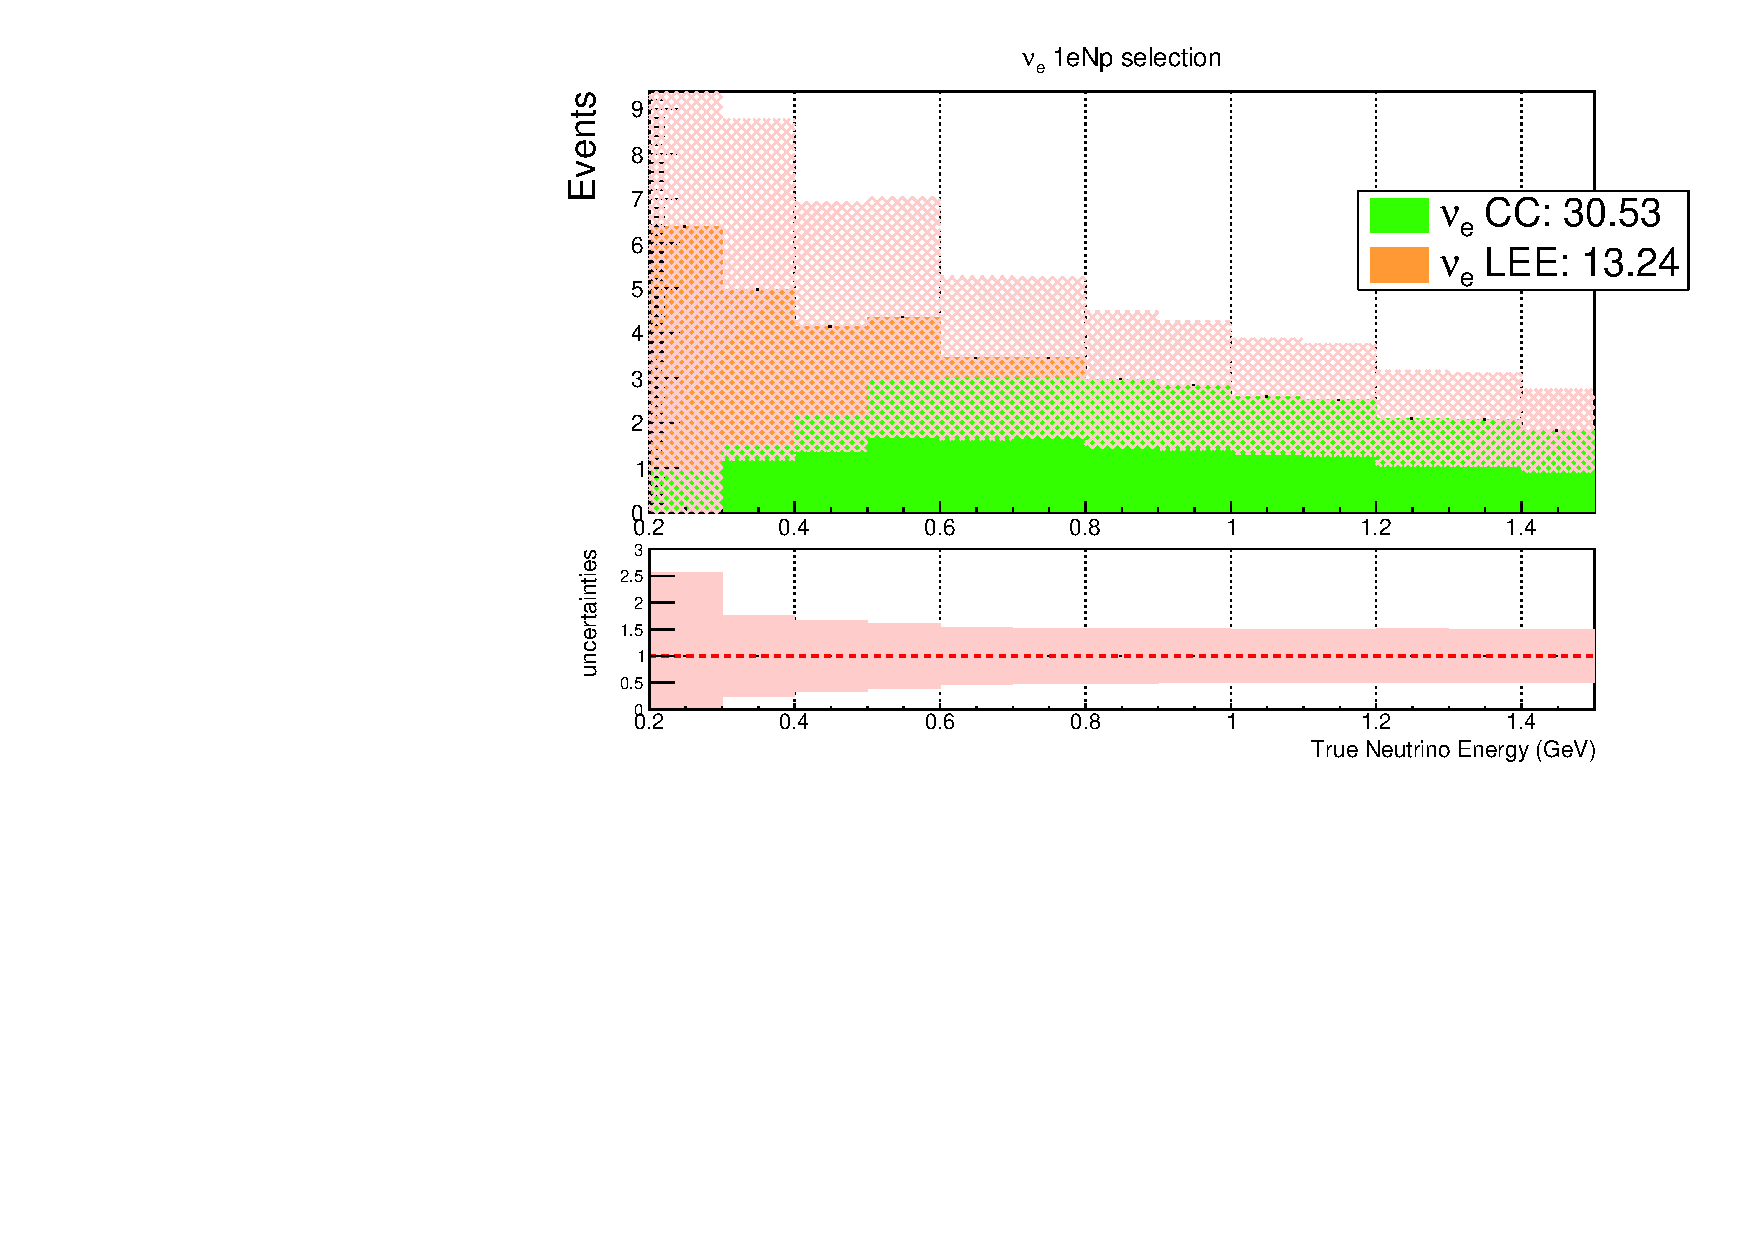
\includegraphics[width=1.00\textwidth]{Sensitivity/numuconstraint-truth/nuenumu_nu_e_truth_1eNp_before_constraint.pdf}
    \caption{before constraint}
    \end{subfigure}
    \begin{subfigure}[b]{0.45\textwidth}
    \centering
    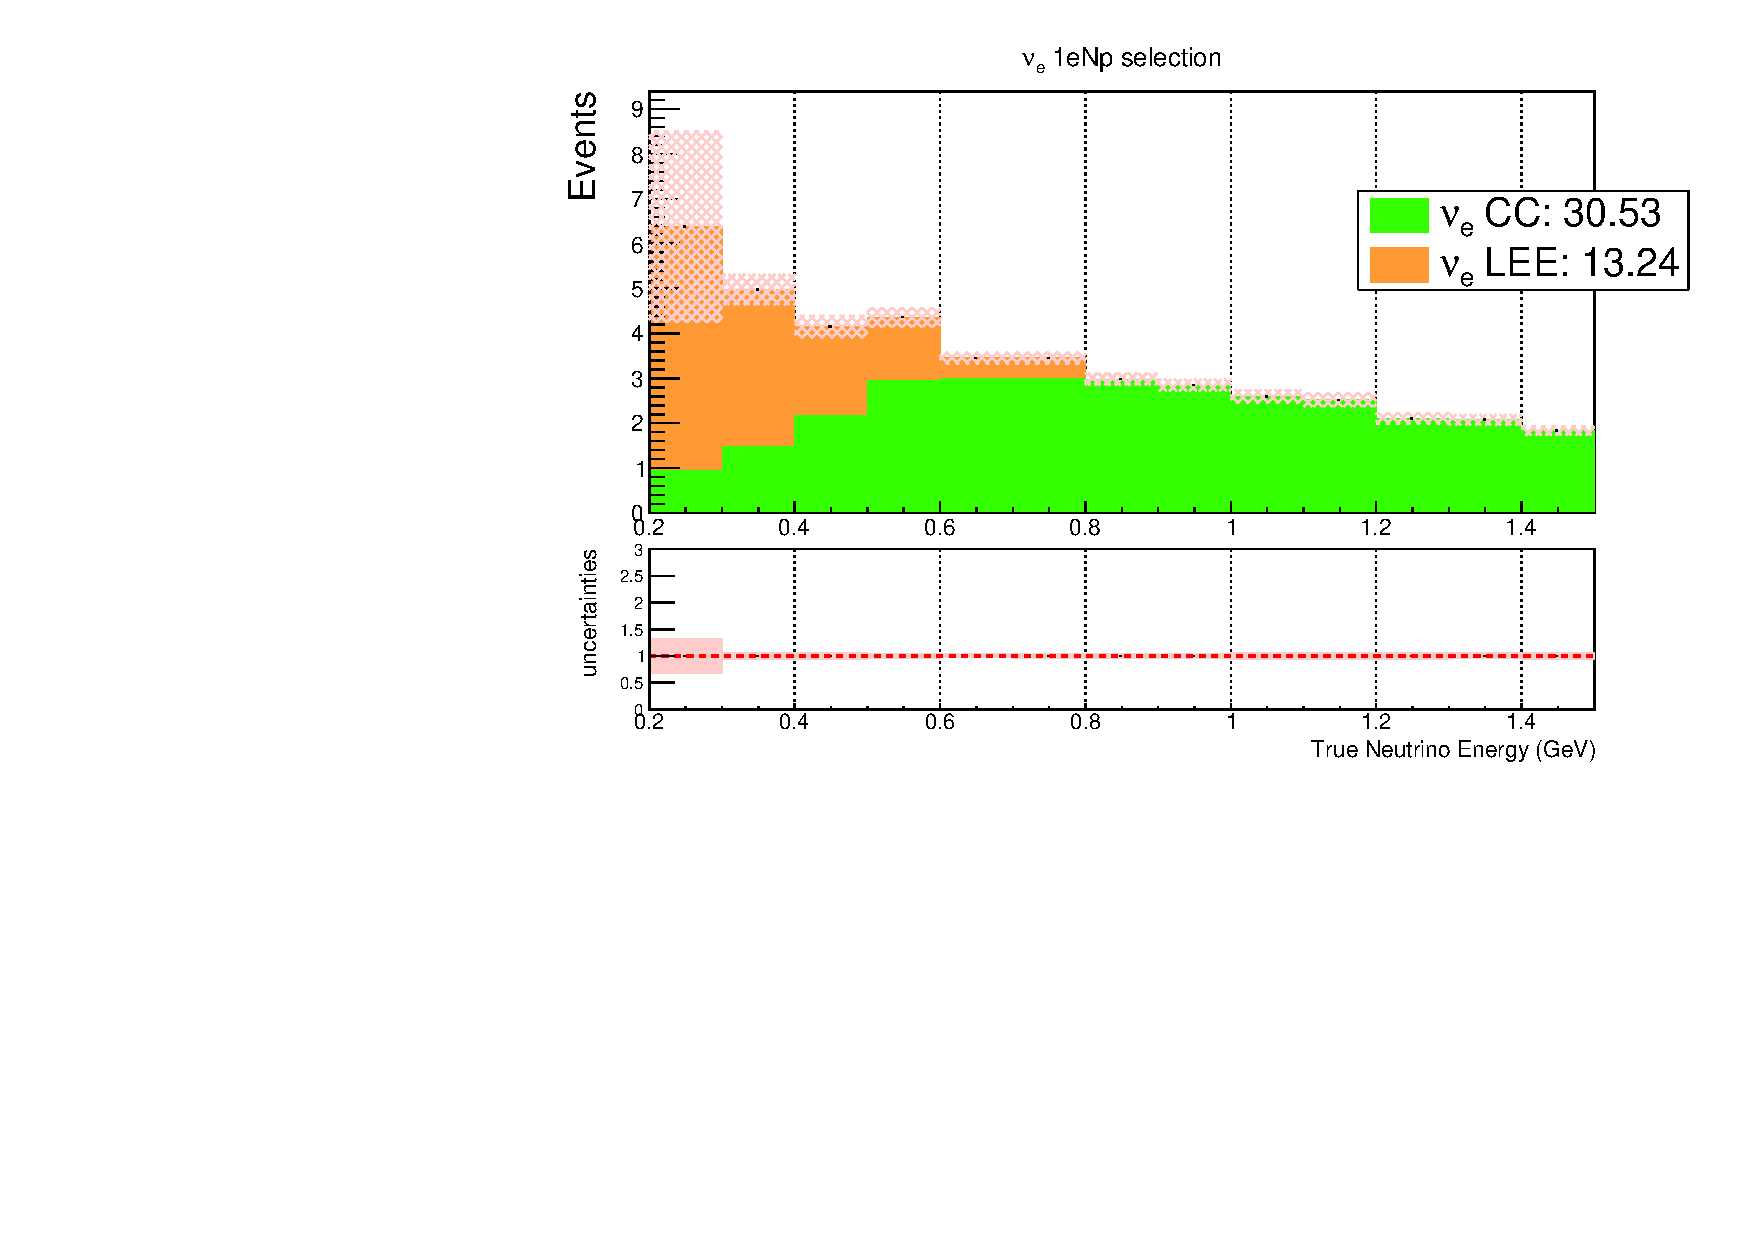
\includegraphics[width=1.00\textwidth]{Sensitivity/numuconstraint-truth/nuenumu_nu_e_truth_1eNp_after_constraint.pdf}
    \caption{after constraint}
    \end{subfigure}
\caption{\label{fig:numuconstraintresult} The truth-level 1eNp selection . The shaded gray band on the top and bottom half of plots (a) and (b) is the systematic uncertainty associated to each bin. Overall we see ~50\% reduction in systematics at the low $\nu_e$ energy bin. \textit{Note that the reduction is only seen in the cross section and flux systematics error, and the MC statistical error is not taken into account}.}
\end{center}
\end{figure}


\begin{center}
\begin{figure}[ht] 
    \begin{subfigure}[b]{0.45\textwidth}
    \centering
    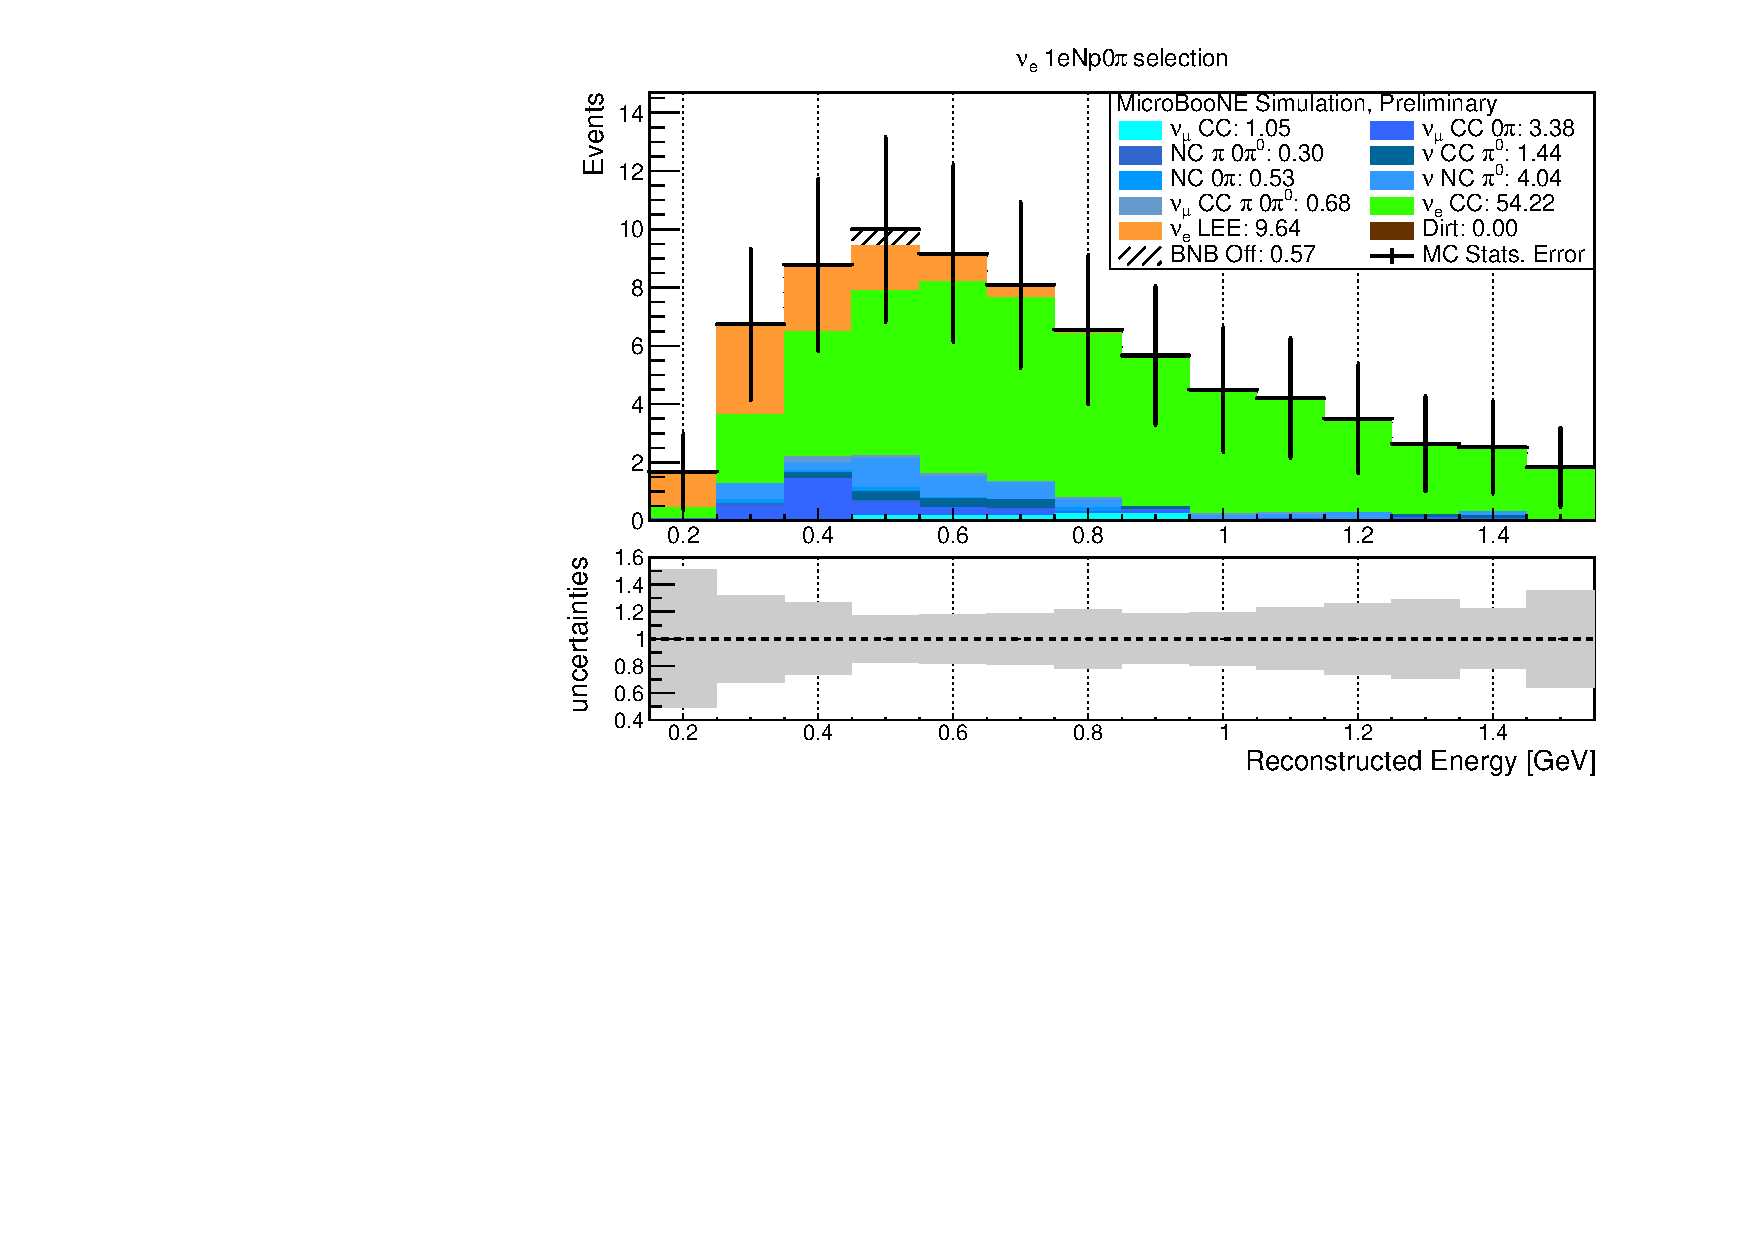
\includegraphics[width=1.00\textwidth]{Sensitivity/newconstraintplots/nue_numu_reco_e_H0_newBDT_higheff_noCCMEC_before_constraint.pdf}
    \caption{before constraint}
    \end{subfigure}
    \begin{subfigure}[b]{0.45\textwidth}
    \centering
    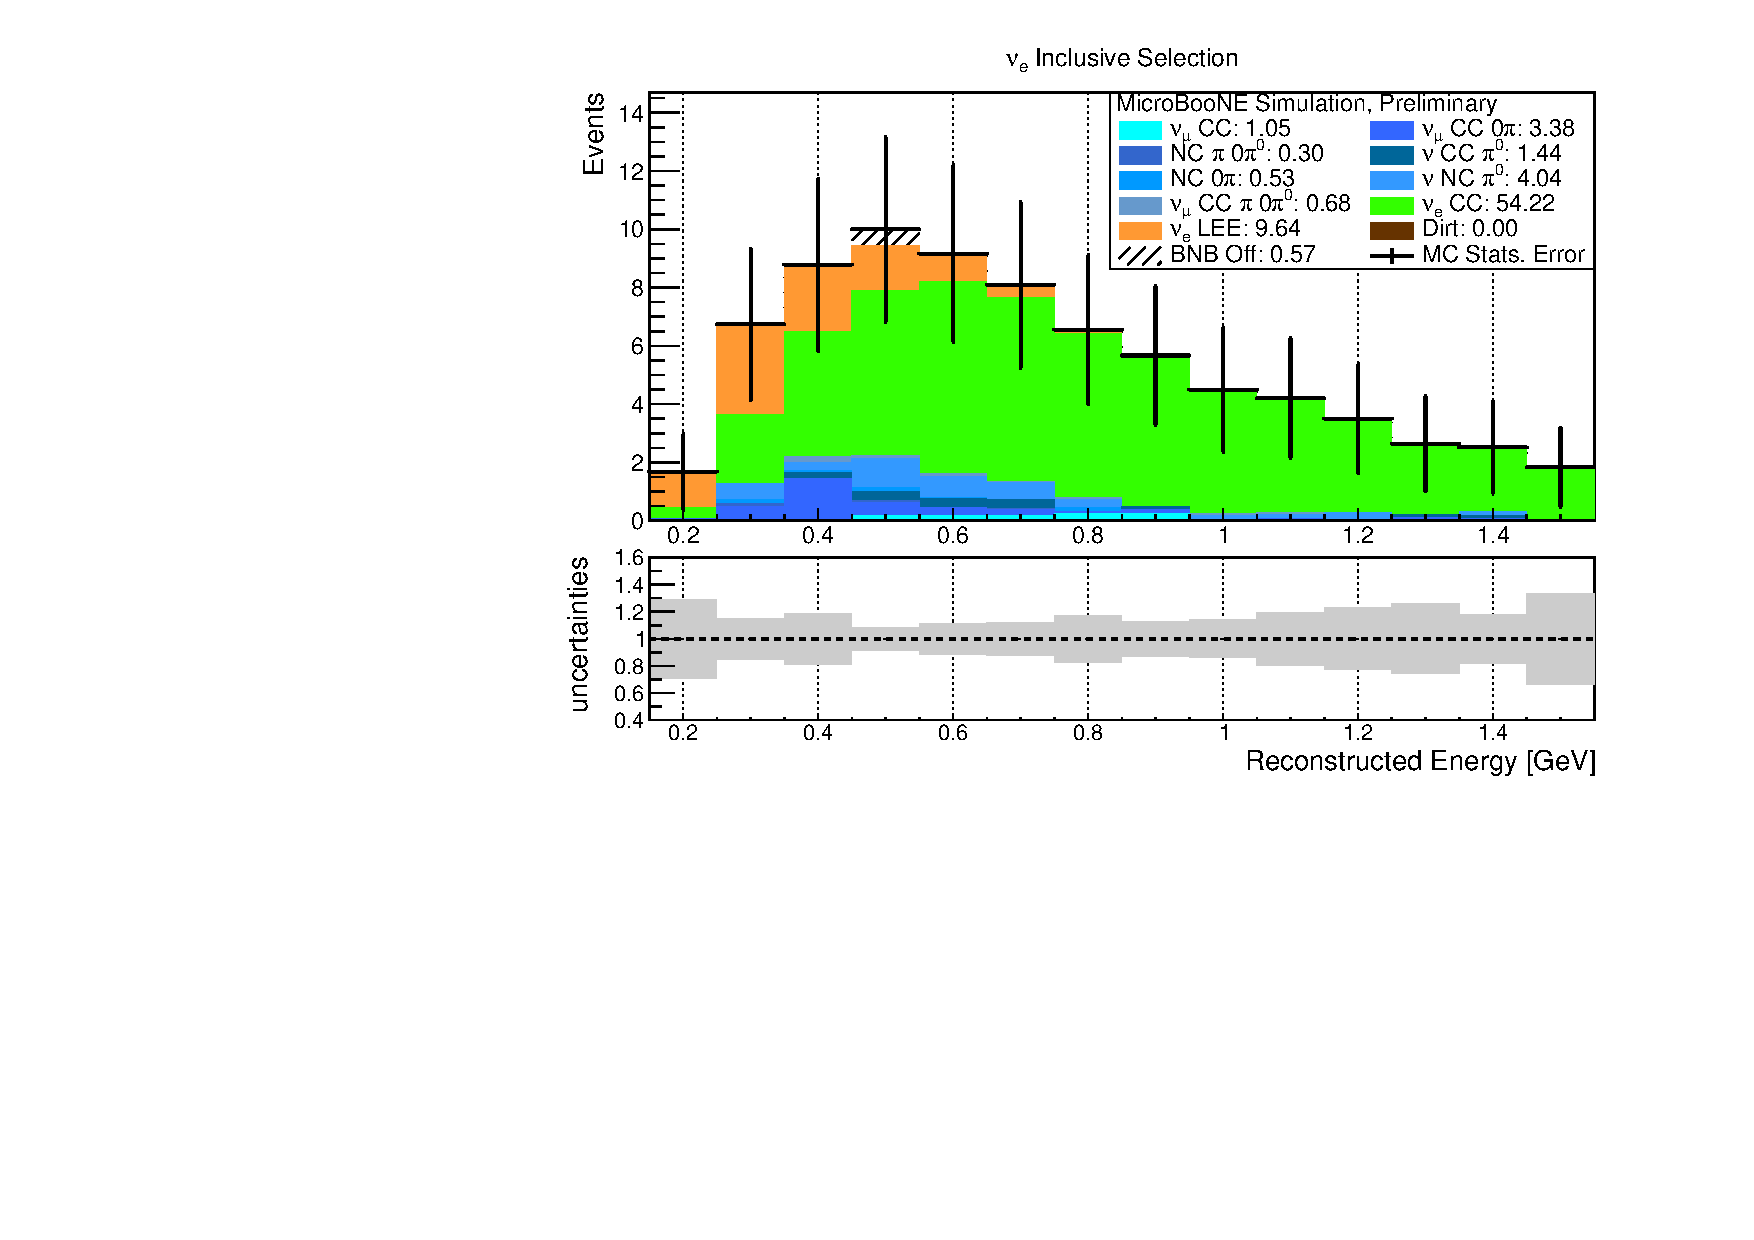
\includegraphics[width=1.00\textwidth]{Sensitivity/newconstraintplots/nue_numu_reco_e_H0_newBDT_higheff_noCCMEC_after_constraint.pdf}
    \caption{after constraint}
    \end{subfigure}
\caption{\label{fig:numuconstraintresultBDTplot} The final \npsel and \zpsel selection from run 1, run 2, and run 3 scaled to $6.95 \times 10^{20}$. The shaded gray band on the top and bottom half of plot (a) and (b) is the systematic uncertainty associated to each bin, and measured with respect to the stacked background plus intrinsic \nue contribution. Overall we see 35\% reduction in systematics at the low $\nu_e$ energy bin.}
\end{figure}
\end{center}
\end{comment}

The quantitative impact of the constraint on diagonal uncertainties in the \npsel reconstructed energy spectrum can be seen in table~\ref{tab:numu_1eNp_bdt_const}.

%\begin{figure}[ht] 
%\begin{center}
%    \begin{subfigure}[b]{0.45\textwidth}
%    \centering
%    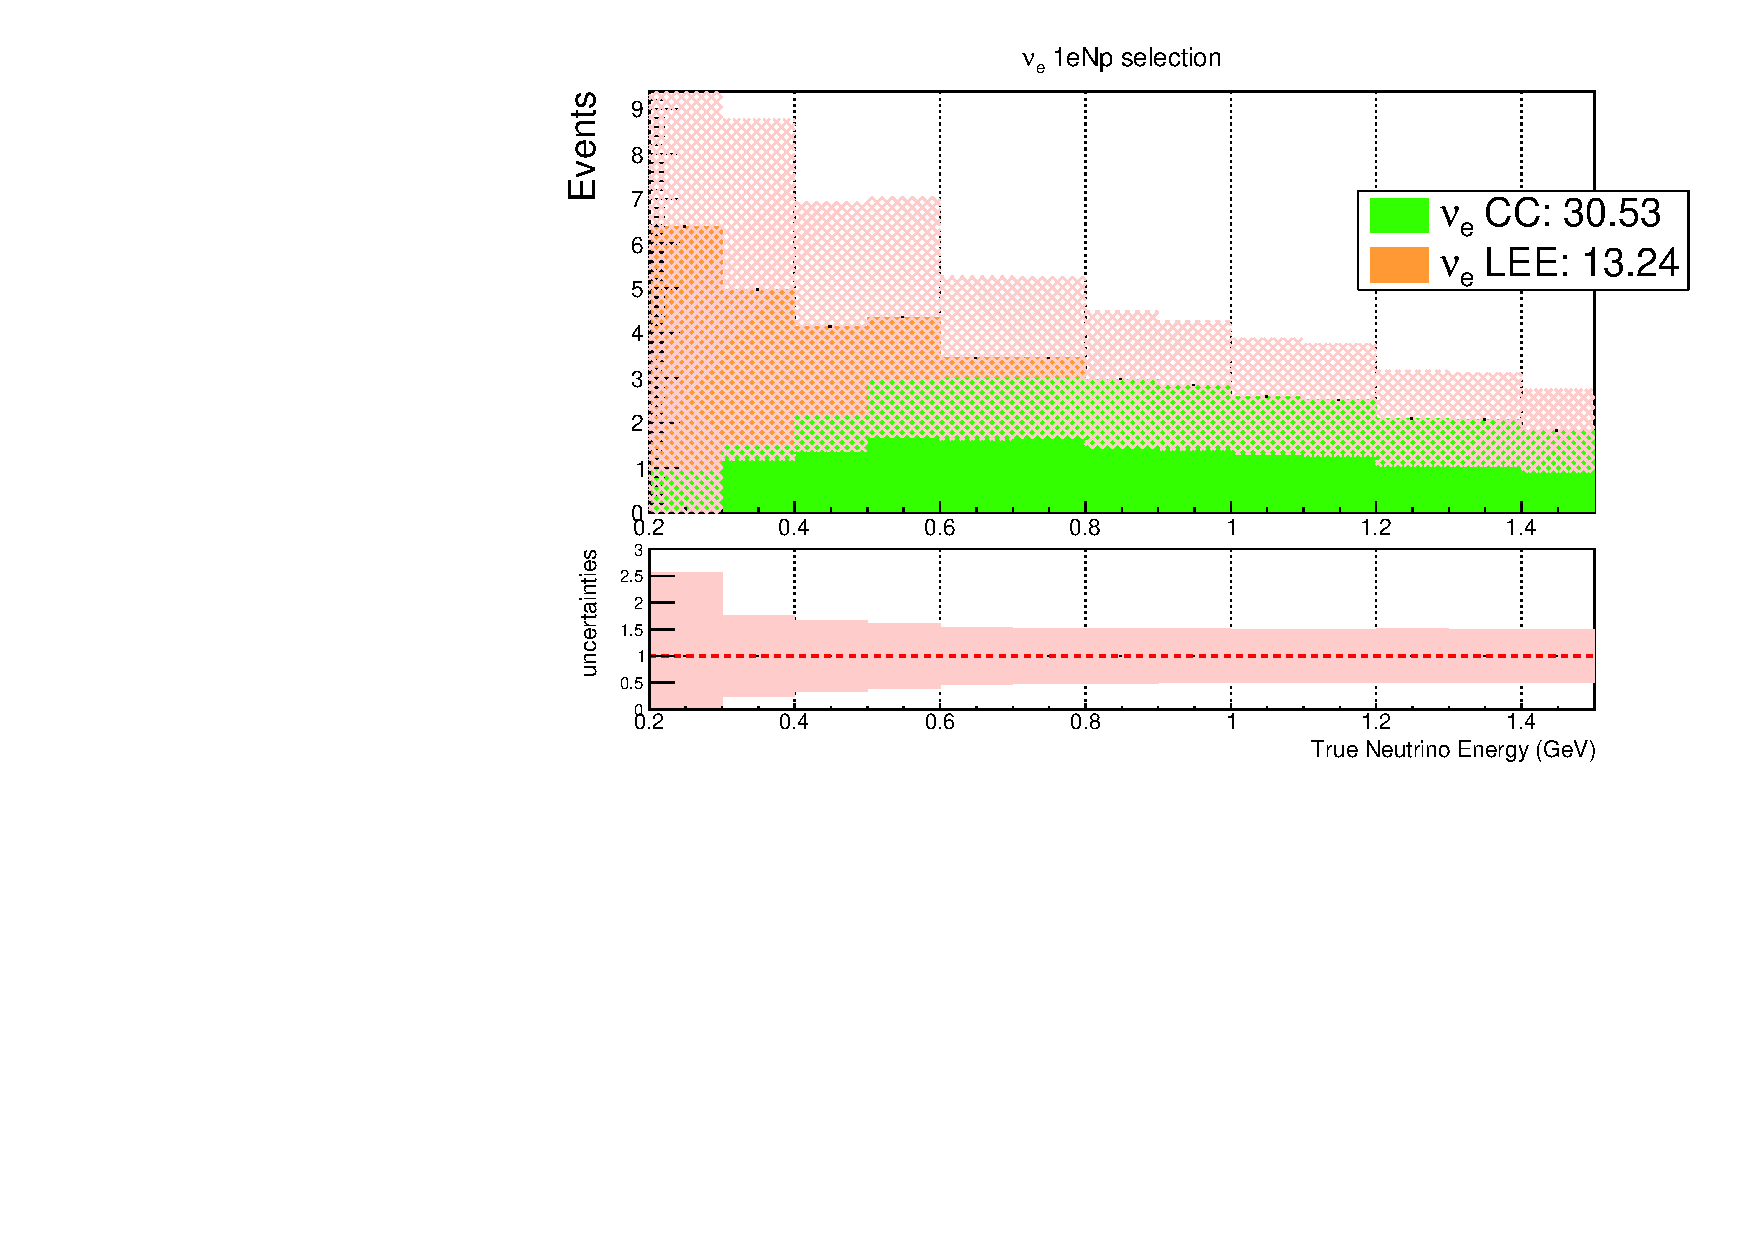
\includegraphics[width=1.00\textwidth]{Sensitivity/numuconstraint-truth/nuenumu_nu_e_truth_1eNp_before_constraint.pdf}
%    \caption{before constraint}
%    \end{subfigure}
%    \begin{subfigure}[b]{0.45\textwidth}
%    \centering
%    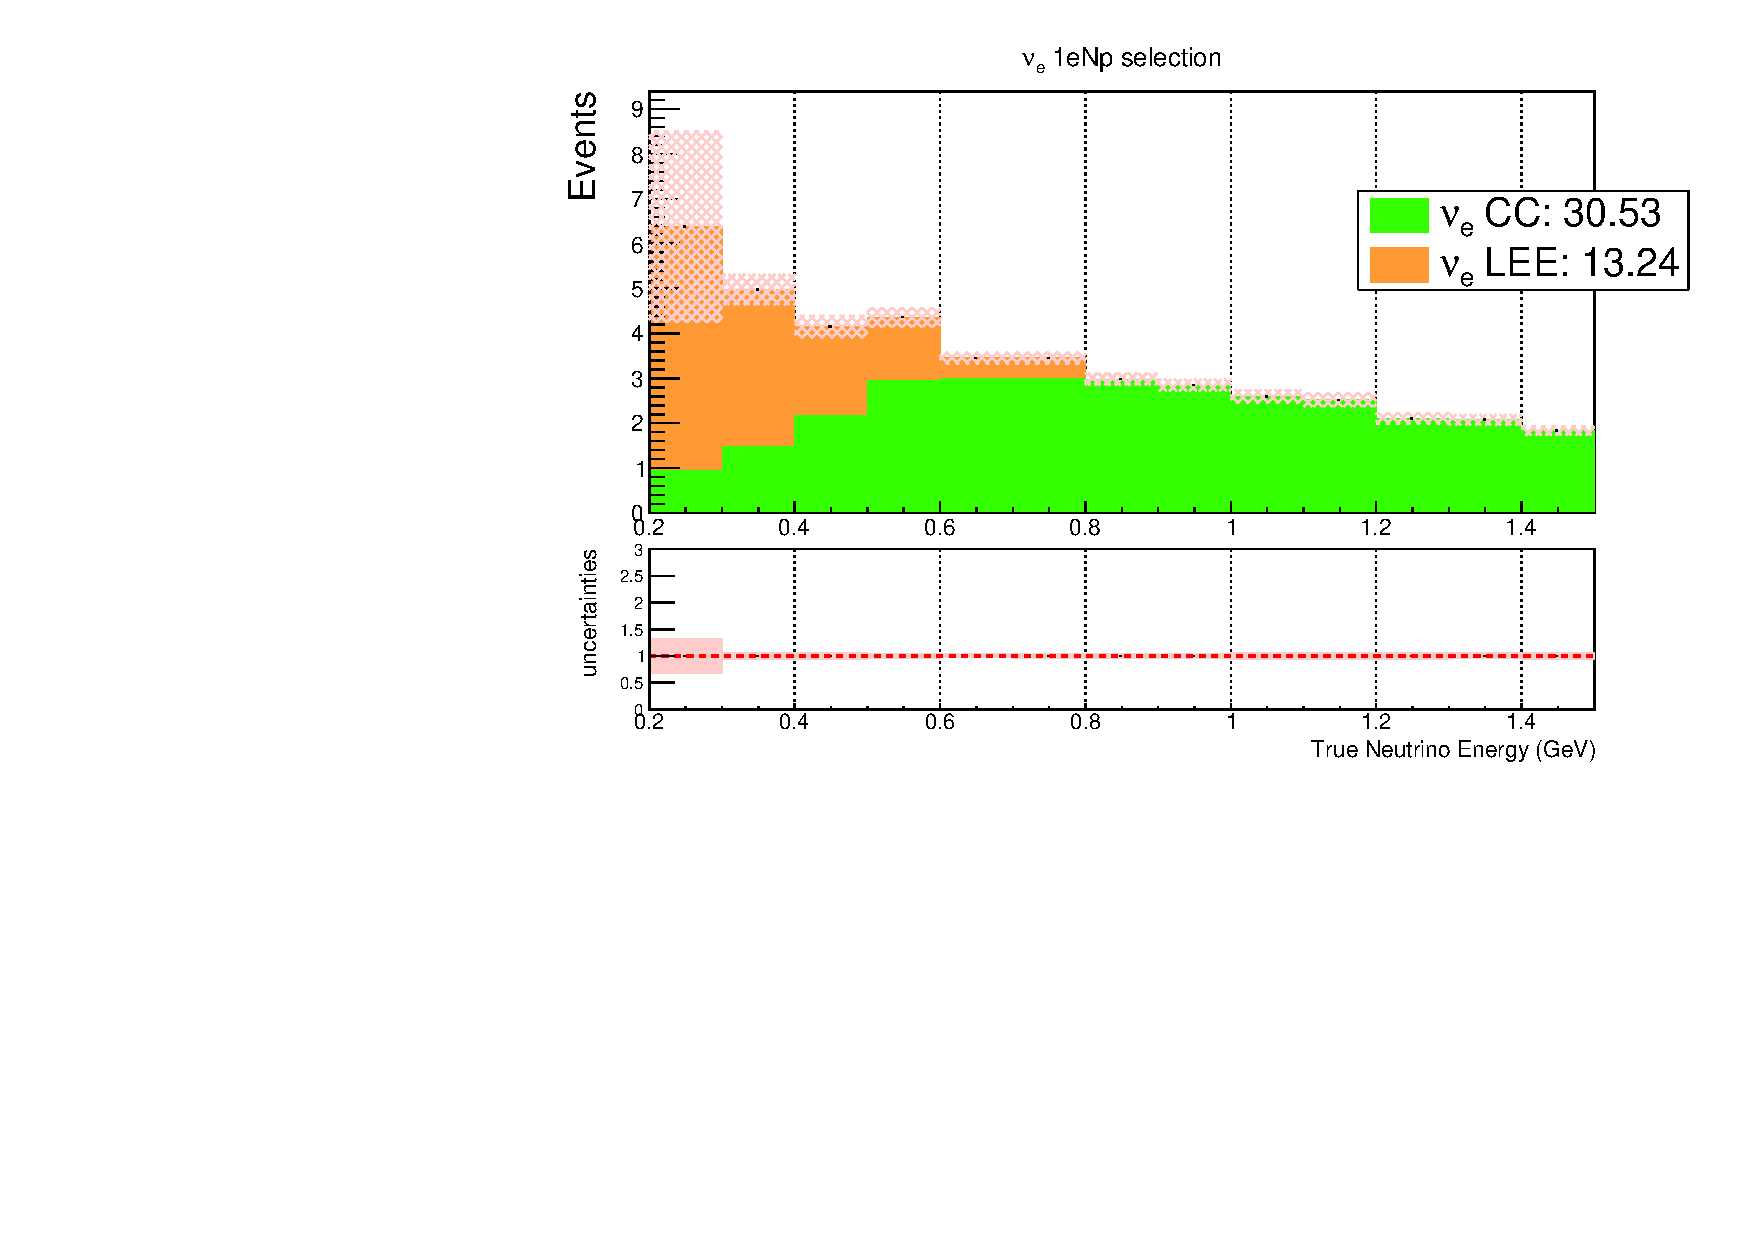
\includegraphics[width=1.00\textwidth]{Sensitivity/numuconstraint-truth/nuenumu_nu_e_truth_1eNp_after_constraint.pdf}
%    \caption{after constraint}
%    \end{subfigure}
%\caption{\label{fig:numuconstraintresult} The truth-level 1eNp selection . The shaded pink band on the top and bottom half of plots (a) and (b) is the systematic uncertainty associated to each bin. Overall we see ~50\% reduction in systematics at the low $\nu_e$ energy bin. \textit{Note that the reduction is only seen in the cross section and flux systematics error, and the MC statistical error is not taken into account}.}
%\end{center}
%\end{figure}

%\subsubsection{Constraint from the \zpsel channel}
%\label{sec:1e0pconstraint}
%\emph{While the procedure to implement the constraints from the \zpsel channel is clear, its results will be shown after the \zpsel selection is optimized.}

%\newpage
%\subsubsection{Summary of the Systematics Constraint}
%\label{subsubsec:sensitivity:constraint_table}

\begin{table}[H]
\centering
\begin{tabular}{| c | m{1.65cm} | m{1.65cm} | m{1.65cm} | m{1.65cm} | m{1.65cm} | m{1.65cm}|}
\cline{1-7}
\multirow{2}{*}{Energy [GeV]} &\multicolumn{3}{c|}{Flux+Genie+G4}&\multicolumn{3}{c|}{Flux+Genie+G4+Det. Systematics}\\
\cline{2-7}
{} &  before constraint & after constraint  & size of reduction & before constraint & after constraint & size of reduction \\
\hline
0.15 - 0.25 & 50.59 & 20.22 & 60.03 & 52.38 & 26.44 & 49.52 \\
0.25 - 0.35 & 34.45 & 8.08 & 76.55 & 35.42 & 12.35 & 65.13 \\
0.35 - 0.45 & 32.29 & 9.18 & 71.57 & 33.23 & 12.85 & 61.33 \\
0.45 - 0.55 & 24.48 & 5.88 & 75.98 & 24.98 & 8.17 & 67.29 \\
0.55 - 0.65 & 23.61 & 5.59 & 76.32 & 24.28 & 8.47 & 65.12 \\
0.65 - 0.75 & 23.10 & 5.72 & 75.24 & 24.02 & 9.41 & 60.82 \\
0.75 - 0.85 & 23.27 & 6.15 & 73.57 & 24.16 & 9.80 & 59.44 \\
0.85 - 0.95 & 22.87 & 6.21 & 72.85 & 24.22 & 10.94 & 54.83 \\
0.95 - 1.05 & 22.04 & 6.00 & 72.78 & 23.84 & 11.51 & 51.72 \\
1.05 - 1.15 & 22.22 & 6.33 & 71.51 & 24.36 & 12.58 & 48.36 \\
1.15 - 1.25 & 21.48 & 7.63 & 64.48 & 32.04 & 25.27 & 21.13 \\
1.25 - 1.35 & 22.25 & 7.17 & 67.78 & 23.69 & 11.52 & 51.37 \\
1.35 - 1.45 & 21.47 & 8.41 & 60.83 & 25.33 & 16.30 & 35.65 \\
1.45 - 1.55 & 21.38 & 7.65 & 64.22 & 27.72 & 19.62 & 29.22 \\   
\hline
\end{tabular}
\caption{Summary of the fractional errors (in percentage) on the flux, genie, and detector systematics before and after the $\nu_\mu$ constrain for the \npsel BDT selection}
\label{tab:numu_1eNp_bdt_const}
\end{table}

\begin{comment}
\begin{table}[H]
\centering
 \begin{tabular}{| c | m{1.65cm} | m{1.65cm} | m{1.65cm} | m{1.65cm} | m{1.65cm} | m{1.65cm}|} 
\cline{1-7}
\multirow{2}{*}{Energy [GeV]} &\multicolumn{3}{c|}{Flux+Genie+G4}&\multicolumn{3}{c|}{Flux+Genie+G4+Det. Systematics}\\
\cline{2-7}
{} &  before constraint & after constraint  & size of reduction & before constraint & after constraint & size of reduction \\
\hline
0.15 - 0.25 & 17.67 & 12.43 & 29.65 & 19.52 & 15.50 & 20.59 \\
0.25 - 0.35 & 19.57 & 8.62 & 55.95 & 20.65 & 11.15 & 46.00 \\
0.35 - 0.45 & 22.73 & 13.38 & 41.14 & 23.69 & 15.43 & 34.87 \\
0.45 - 0.55 & 14.97 & 7.28 & 51.37 & 15.95 & 9.29 & 41.76 \\
0.55 - 0.65 & 29.74 & 13.54 & 54.47 & 33.27 & 20.56 & 38.20 \\
0.65 - 0.75 & 27.02 & 14.91 & 44.82 & 30.01 & 20.59 & 31.39 \\
0.75 - 0.85 & 23.00 & 12.16 & 47.13 & 25.94 & 17.42 & 32.85 \\
0.85 - 0.95 & 19.06 & 9.00 & 52.78 & 23.65 & 16.88 & 28.63 \\
0.95 - 1.05 & 31.24 & 15.59 & 50.10 & 45.36 & 36.68 & 19.14 \\
1.05 - 1.15 & 33.30 & 19.48 & 41.50 & 46.80 & 38.53 & 17.67 \\
1.15 - 1.25 & 31.29 & 17.21 & 45.00 & 35.70 & 24.80 & 30.53 \\
1.25 - 1.35 & 33.32 & 22.54 & 32.35 & 37.49 & 28.77 & 23.26 \\
1.35 - 1.45 & 14.07 & 7.89 & 43.92 & 16.13 & 11.41 & 29.26 \\
1.45 - 1.55 & 20.43 & 10.48 & 48.70 & 24.61 & 17.54 & 28.73 \\
\hline
\end{tabular}
\caption{Summary of the fractional errors (in percentage) on the flux, genie, and detector systematics before and after the $\nu_\mu$ and 1e0p$0\pi$ constrain for the BDT selection}
\label{tab:numu_1e0p_bdt_const}
\end{table}

\begin{table}[H]
\centering
 \begin{tabular}{| c | m{1.65cm} | m{1.65cm} | m{1.65cm} | m{1.65cm} | m{1.65cm} | m{1.65cm}|} 
\cline{1-7}
\multirow{2}{*}{Energy [GeV]} &\multicolumn{3}{c|}{Flux+Genie}&\multicolumn{3}{c|}{Flux+Genie+Det. Systematics}\\
\cline{2-7}
{} &  before constraint & after constraint  & size of reduction & before constraint & after constraint & size of reduction \\
\hline
0.15 - 0.25&47.96&24.15&49.65&50.84&37.70&25.85\\
0.25 - 0.35&30.24&10.40&65.61&32.30&18.76&41.92\\
0.35 - 0.45&19.77&7.37&41.01&26.48&19.83&25.11\\
0.45 - 0.55&15.83&4.58&37.20&17.20&8.72&49.30\\
0.55 - 0.65&15.18&5.31&32.64&18.17&11.79&35.11\\
0.65 - 0.75&15.58&5.22&34.26&18.89&12.32&34.78\\
0.75 - 0.85&14.32&6.06&27.31&21.72&17.80&18.05\\
0.85 - 0.95&15.31&6.90&27.81&18.33&13.40&26.90\\
0.95 - 1.05&15.45&6.74&28.80&19.55&14.32&26.75\\
1.05 - 1.15&14.85&7.72&23.58&22.85&19.77&13.48\\
1.15 - 1.25&15.72&8.40&24.21&26.12&23.08&11.64\\
1.25 - 1.35&16.53&8.48&26.62&29.17&26.19&10.22\\
1.35 - 1.45&16.81&9.83&23.08&22.21&18.33&17.47\\
1.45 - 1.55&15.24&7.57&25.36&35.90&33.78&5.91\\
\hline
\end{tabular}
\caption{Summary of the fractional errors (in percentage) on the flux, genie, and detector systematics before and after the $\nu_\mu$ and 1e0p$0\pi$ constrain for the \npsel BDT selection}
\label{tab:numu_1e0p_bdt_const}
\end{table}
\end{comment}

\subsubsection{Constraint from \numu selections on the \zpsel selection}
\label{subsec:zpselconstraint}

\par We follow the same procedures as described in Section~\ref{subsec:constraintfromnumu} and perform the \numu constraint to the \zpsel selection via the covariance matrix. Again, we make an assumption that the $N_{MC}$ is approximately the same as the $N_{signal}$ for the \numu constraint channel. The constraint technique leads to, in this exercise, a reduction in systematic uncertainties of $\sim50$\% if we are only folding in the correlated flux, genie, and geant-4 systematics, and $\sim35$\% when we include the uncorrelated detector systematics.
Figure~\ref{fig:numuconstraintzpselnpsel} shows the effects of the $\nu_\mu$ constraint on the systematics of the \zpsel $\nu_e$ selections.

\begin{center}
\begin{figure}[ht] 
    \begin{subfigure}{0.45\textwidth}
    \centering
    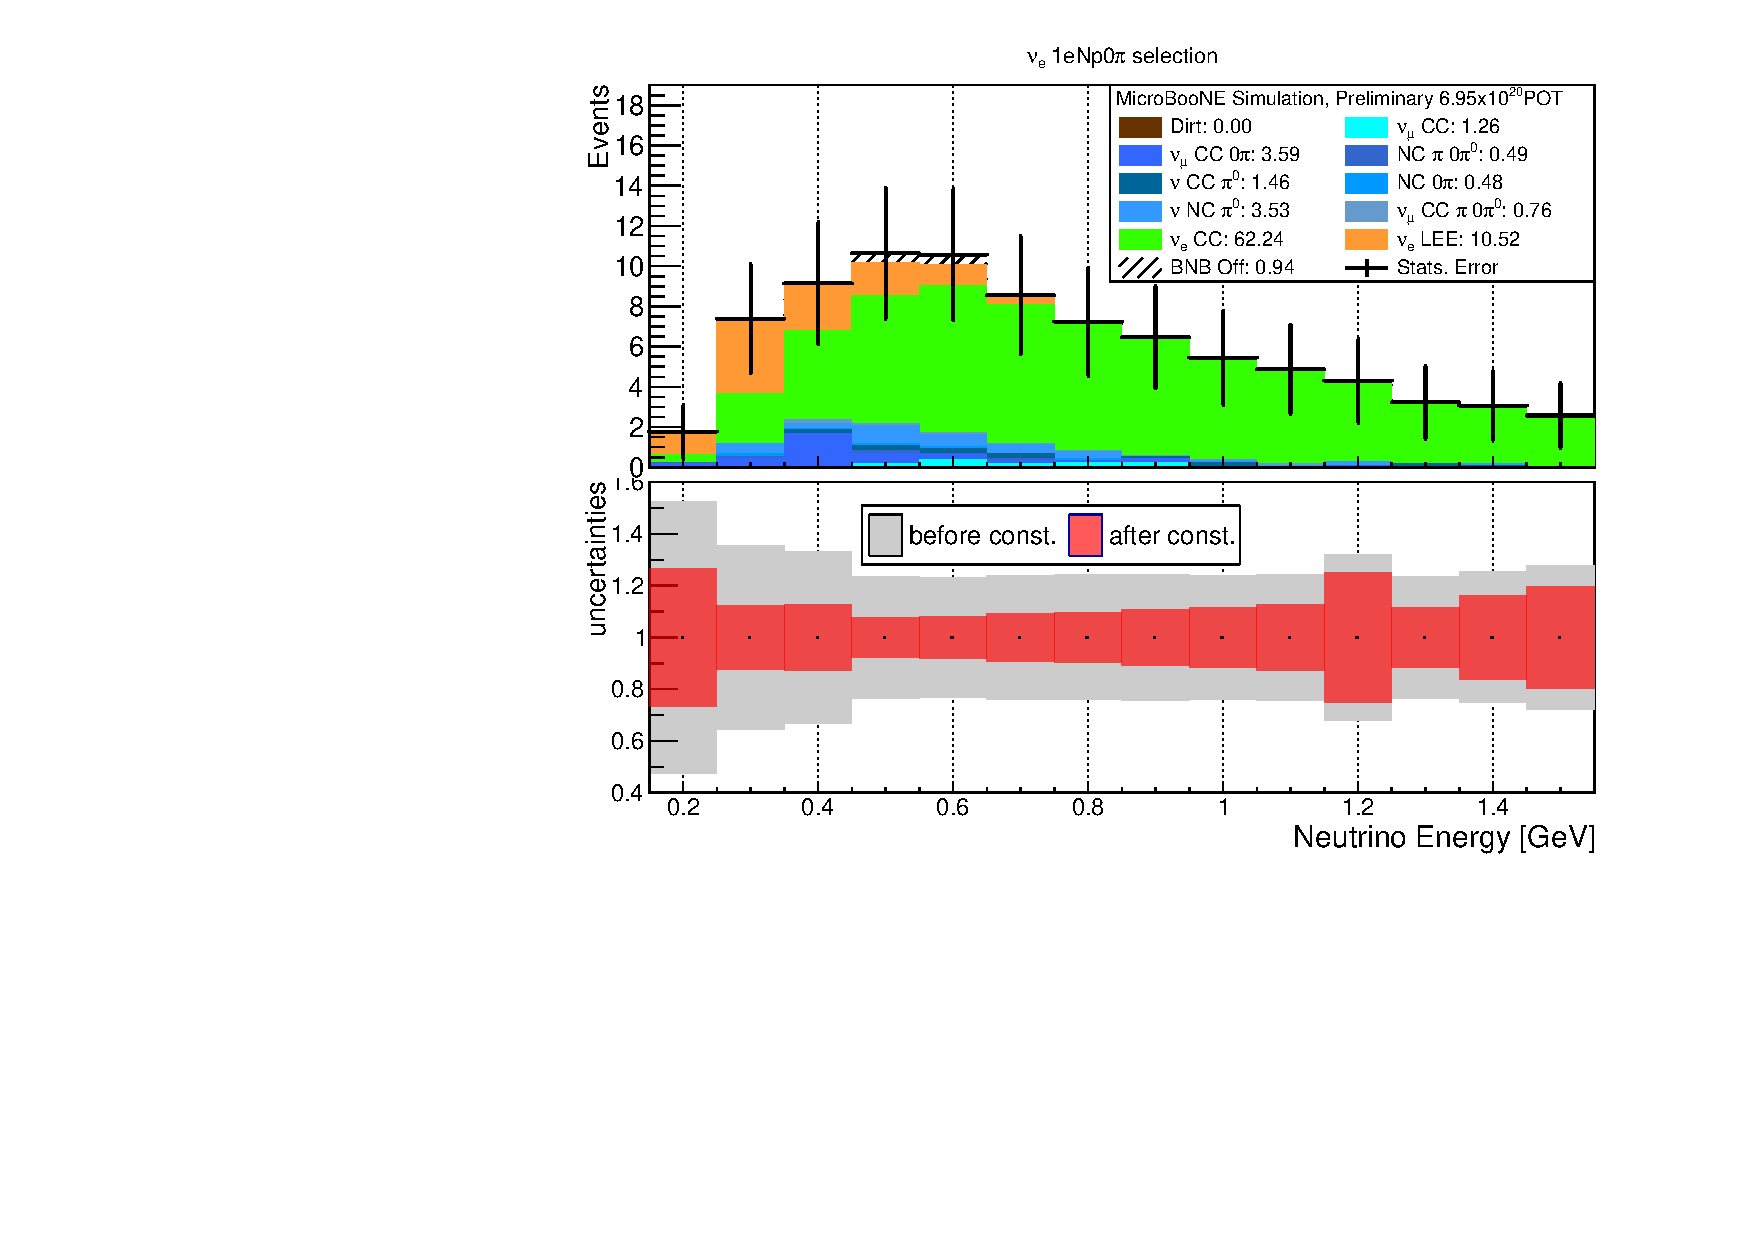
\includegraphics[width=1.00\textwidth]{Sensitivity/newconstraintplots/nue_numu_reco_e_H1_mc_collab_beforeafter_constraint.pdf}
    \caption{\npsel selection}
    \end{subfigure}
    \begin{subfigure}{0.45\textwidth}
    \centering
    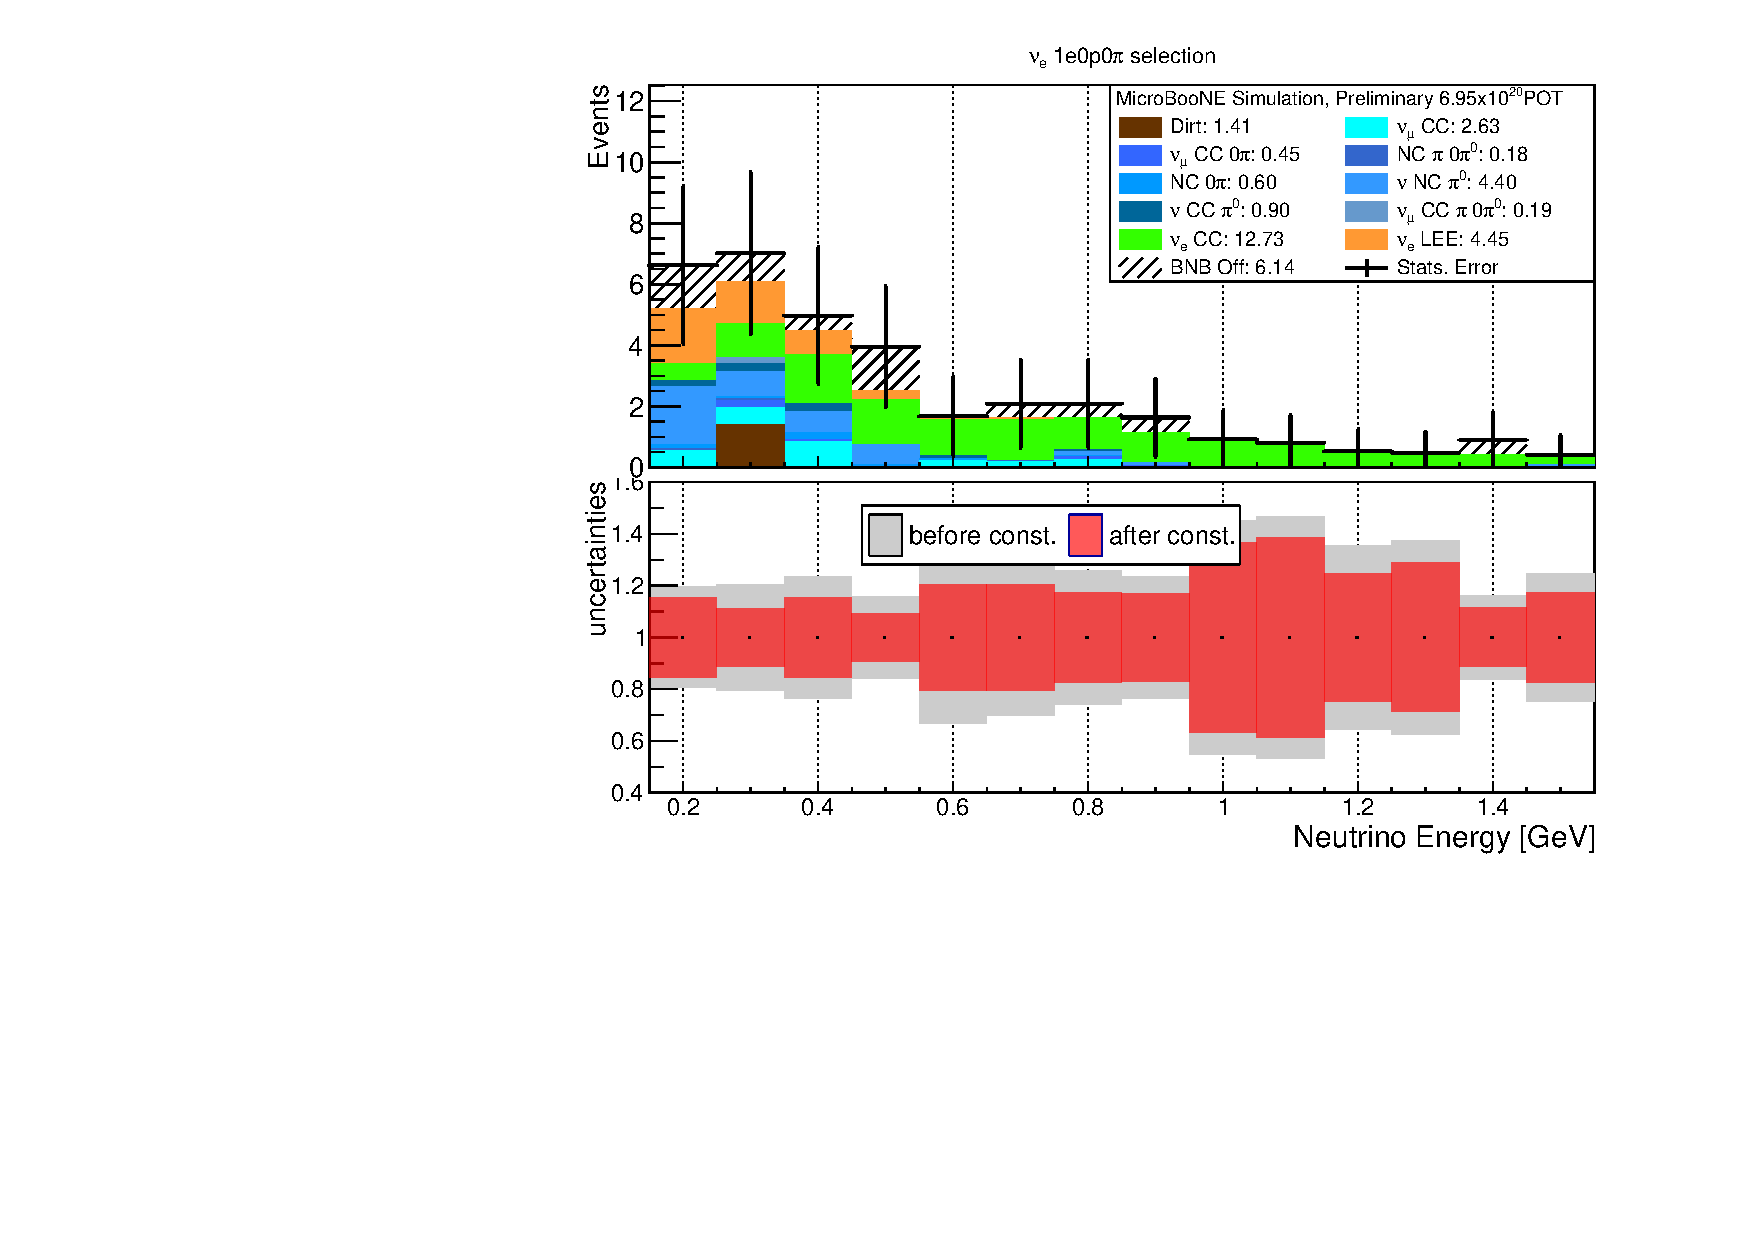
\includegraphics[width=1.00\textwidth]{Sensitivity/newconstraintplots/1e0p_numu_reco_e_H1_mc_collab_beforeafter_constraint.pdf}
    \caption{\zpsel selection}
    \end{subfigure}
\caption{\label{fig:numuconstraintzpselnpsel} The final \npsel and \zpsel selection from run 1, run 2, and run 3 scaled to $6.95 \times 10^{20}$. The shaded gray and pink band on the bottom half of plots (a) and (b) is respectively the systematic uncertainty associated to each bin, before and after the \numu constraint, and measured with respect to the stacked background plus intrinsic \nue only contribution. The size of the reduction in each bin for selection (a) and (b) is given in ~\cref{tab:numu_1eNp_bdt_const} and ~\cref{tab:numu_1e0p_bdt_const}, respectively.}
\end{figure}
\end{center}
The quantitative impact of the constraint on diagonal uncertainties in the \zpsel reconstructed energy spectrum can be seen in table~\ref{tab:numu_1e0p_bdt_const}.

\begin{table}[H]
\centering
\begin{tabular}{| c | m{1.65cm} | m{1.65cm} | m{1.65cm} | m{1.65cm} | m{1.65cm} | m{1.65cm}|}
\cline{1-7}
\multirow{2}{*}{Energy [GeV]} &\multicolumn{3}{c|}{Flux+Genie+G4}&\multicolumn{3}{c|}{Flux+Genie+G4+Det. Systematics}\\
\cline{2-7}
{} &  before constraint & after constraint  & size of reduction & before constraint & after constraint & size of reduction \\
\hline
0.15 - 0.25 & 25.05 & 17.53 & 30.02 & 27.66 & 21.94 & 20.68 \\
0.25 - 0.35 & 23.45 & 10.29 & 56.12 & 24.74 & 13.35 & 46.04 \\
0.35 - 0.45 & 25.70 & 15.11 & 41.21 & 26.79 & 17.44 & 34.90 \\
0.45 - 0.55 & 24.53 & 11.90 & 51.49 & 26.14 & 15.23 & 41.74 \\
0.55 - 0.65 & 29.74 & 13.48 & 54.67 & 33.27 & 20.55 & 38.23 \\
0.65 - 0.75 & 34.81 & 19.03 & 45.33 & 38.66 & 26.50 & 31.45 \\
0.75 - 0.85 & 29.37 & 15.48 & 47.29 & 33.13 & 22.24 & 32.87 \\
0.85 - 0.95 & 27.13 & 12.75 & 53.00 & 33.66 & 24.01 & 28.67 \\
0.95 - 1.05 & 31.24 & 15.54 & 50.26 & 45.36 & 36.67 & 19.16 \\
1.05 - 1.15 & 33.30 & 19.43 & 41.65 & 46.80 & 38.52 & 17.69 \\
1.15 - 1.25 & 31.29 & 17.16 & 45.16 & 35.70 & 24.79 & 30.56 \\
1.25 - 1.35 & 33.32 & 22.49 & 32.50 & 37.49 & 28.76 & 23.29 \\
1.35 - 1.45 & 30.68 & 17.12 & 44.20 & 35.17 & 24.87 & 29.29 \\
1.45 - 1.55 & 20.43 & 10.44 & 48.90 & 24.61 & 17.53 & 28.77 \\
\hline
\end{tabular}
\caption{Summary of the fractional errors (in percentage) on the flux, genie, and detector systematics before and after the $\nu_\mu$ constrain for the \zpsel BDT selection}
\label{tab:numu_1e0p_bdt_const}
\end{table}

\subsection{Final Sensitivities}

\par The sensitivity to the MB-\nue LEE model is computed by constructing a combined matrix of \npsel, \zpsel, and \numu channels as described in ~\cref{ssec:finalSensitivityCalc}. This combined matrix is then fed into ~\cref{eqn:deltachi2_systematic}, where the inclusion of the \numu channel will effectively constrain the systematics of the \npsel and \zpsel channels through the correlation elements between the channels of the covariance matrix. In addition, the incorporation of the \zpsel selection also provide additional constraint for the uncertainty related to proton reconstruction, multiplicity and kinematics in the \npsel selection through the side-by-side fit.

%leveraging the constraint procedure of sec.~\ref{subsec:constraintfromnumu} and utilizing the constrained covariance matrix summarized by table~\ref{tab:numu_1e0p_bdt_const} as input, the sensitivity to the MB-\nue LEE model is computed and illustrated in figure~\ref{fig:constrained_sensitivity}. 
A summary of the measured sensitivity for the BDT selections with stats-only, systematics, and constrained systematics is presented in table~\ref{tab:sensitivity}. Supplemental plots for the sensitivity estimation using the expected 12.5E20POT from run 1-5 is given in ~\cref{app:sensitivity}.

\begin{table}[H]
\centering
\setlength{\tabcolsep}{10pt}
\renewcommand{\arraystretch}{1.25}
 \begin{tabular}{| c | c | c | m{2.3 cm} | c | c | c |} 
 \hline
 POT & LEE events & \nue events & scenario & stat. $\sigma$  & stat+syst. $\sigma$ & constrained $\sigma$ \\
 \hline
\multirow{2}{*}{$6.95E20$} &  \multirow{2}{*}{14.97} & \multirow{2}{*}{74.97} & ruling out SM if LEE is true & $2.5$ & $1.9$ & $2.3$ \\
 &  &  & ruling out LEE if SM is true & $2.2$ & $1.9$ & $2.2$ \\
\multirow{2}{*}{$12.5E20$} & \multirow{2}{*}{26.91} & \multirow{2}{*}{134.85} & ruling out SM if LEE is true & $3.3$ & $2.3$ & $3.0$ \\
 &  &  & ruling out LEE if SM is true &$3.0$ & $2.5$ & $2.9$ \\
 \hline
 \end{tabular}
 \caption{\label{tab:sensitivity}Expected sensitivity for run 1-3 data and the run 1-5 data. Event counts are scaled to $6.95E20$ POT and 12.5E20 and include both \npsel and \zpsel LEE signal events.}
\end{table}


\begin{comment}
\begin{table}[H]
\centering
\setlength{\tabcolsep}{10pt}
\renewcommand{\arraystretch}{1.25}
 \begin{tabular}{| c | c | c | c | c | c |} 
 \hline
 channel & LEE events & \nue events & stat. $\sigma$  & stat+syst. $\sigma$ & constrained $\sigma$ \\
 \hline
box-cut \npsel & 10.6 & 51.6 & $2.7$ & $2.3$ & $2.5$ \\
BDT-based \npsel & 14.1 & 74.7 & $2.8$ & $2.3$ & $2.6$ \\
 \hline
 \end{tabular}
 \caption{\label{tab:sensitivity}Expected sensitivity for the Box-Cut and BDT selections of the analysis. Event counts are scaled to $10.1E20$ POT.}
\end{table}
\end{comment}

\begin{figure}[H]
    \begin{center}
    \begin{comment}
    \begin{subfigure}{0.45\textwidth}
    \includegraphics[width=1.00\textwidth]{Sensitivity/sensitivity-run123/SBNfit_Cls_nue_1e0p_numu_reco_e_H1_mc_collab_systCNP_Chi.pdf}
    \label{fig:sensitivity_boxcut_const}
    \caption{Box Cut selection}
    \end{subfigure}
    \end{comment}
    \begin{comment}
    \begin{subfigure}{0.45\textwidth}
    \includegraphics[width=1.00\textwidth]{Sensitivity/sensitivity-run123/SBNfit_Cls_nue_1e0p_numu_reco_e_H1_mc_collab_syst_exclusionCNP_Chi.pdf}
    \label{fig:sensitivity_bdt_const}
    \caption{BDT selection}
    \end{subfigure}
    \end{comment}
    \begin{subfigure}{0.45\textwidth}
    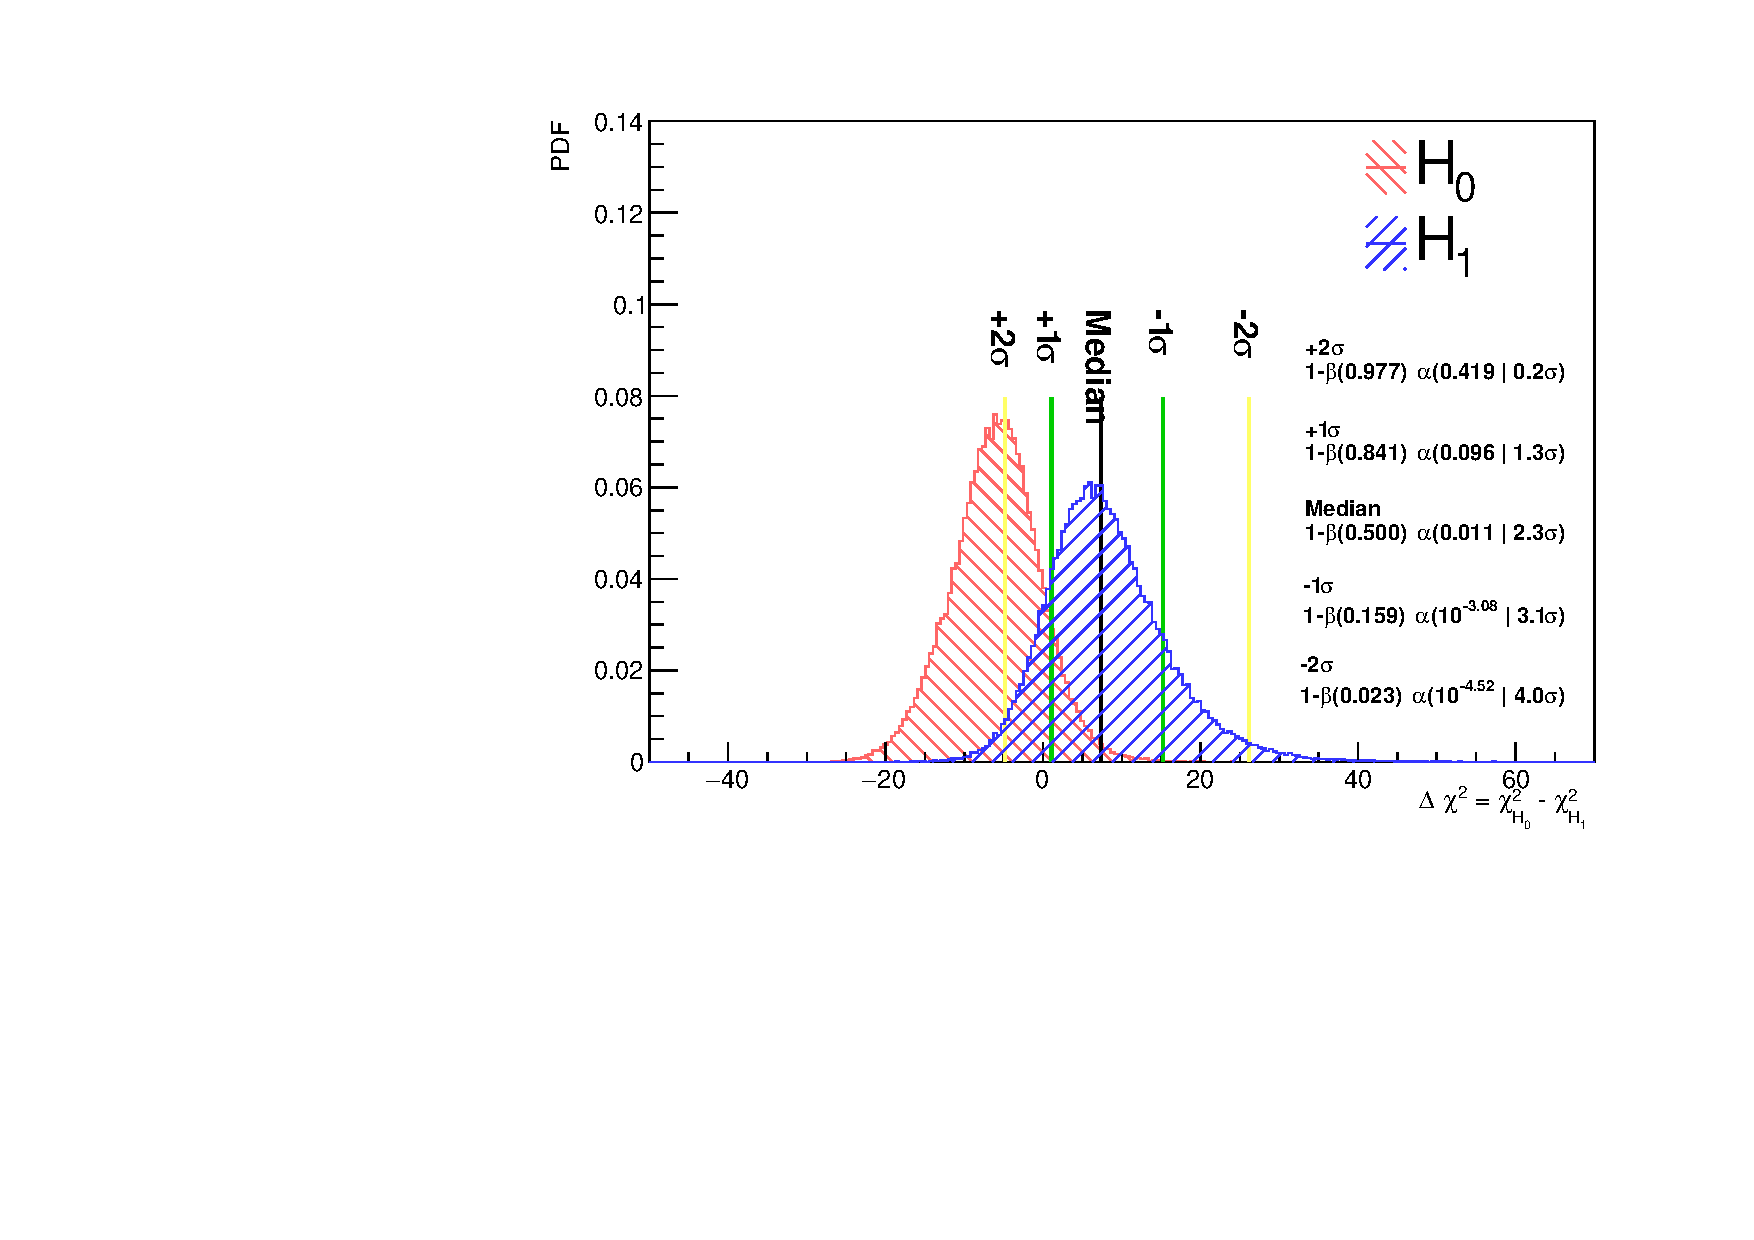
\includegraphics[width=1.00\textwidth]{Sensitivity/sensitivity-run123/SBNfit_Cls_nue_1e0p_numu_reco_e_H1_mc_collab_syst_detsysCNP_Chi.pdf}
    \label{fig:sensitivity_bdt_loose_const}
    \caption{ruling out SM if LEE is true}
    \end{subfigure}
    \begin{subfigure}{0.45\textwidth}
    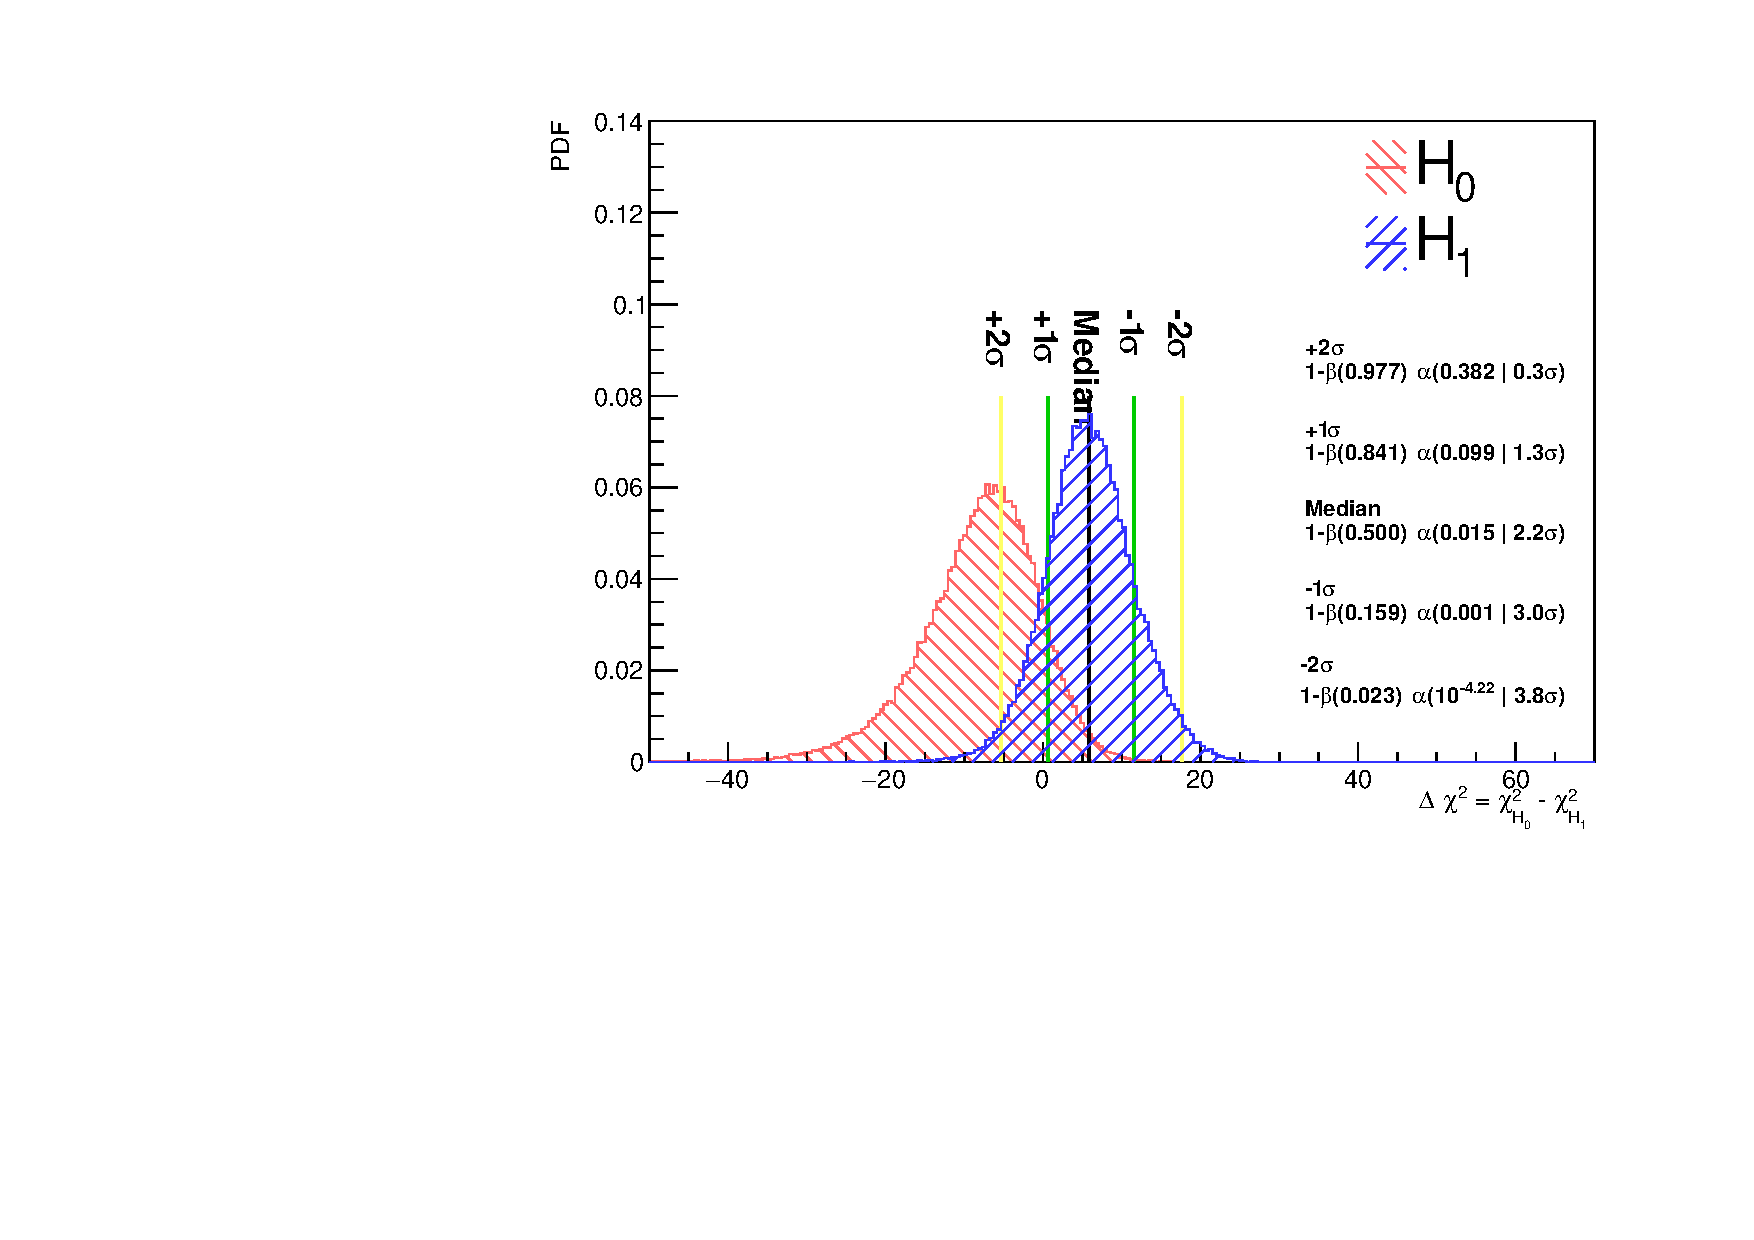
\includegraphics[width=1.00\textwidth]{Sensitivity/sensitivity-run123/SBNfit_Cls_nue_1e0p_numu_reco_e_H1_mc_collab_syst_detsys_exclusionCNP_Chi.pdf}
    \label{fig:sensitivity_bdt_loose_const}
    \caption{ruling out LEE if SM is true}
    \end{subfigure}
    \caption{\label{fig:constrained_sensitivity}Final discovery sensitivity to the LEE unfolded signal of the \npsel and \zpsel selection with constrained systematics. Sample is taken from combined Monte Carlo samples of Run 1, Run 2, and Run 3 and scaled to $6.95\times10^20$ POT.  (a) $H_0$ is the standard model and $H_1$ is the LEE model, (b) $H_0$ is the LEE model and $H_1$ is the standard model.}
    \end{center}
\end{figure}


\begin{comment}
\subsection{Final Exclusion Sensitivities }
We also study exclusion sensitivities of the LEE model by generating fake data under both hypothesis $H_0$ and $H_1$. In this exclusion study, $H_0$ is the distribution of the fake data under the LEE hypothesis and $H_1$ is the distribution of the fake data under the null hypothesis. The $\chi^2$ distribution for each fake data points is computed using the $\Delta \chi^2$ test statistics defined in Eq.~\ref{eqn:deltachi2_systematic}.

\begin{table}[H]
\centering
\setlength{\tabcolsep}{10pt}
\renewcommand{\arraystretch}{1.25}
 \begin{tabular}{| c | c | c | c | c |} 
 \hline
 channel & signal events / $10.1E20$ POT & stat. $\sigma$  & stat+syst. $\sigma$ & constrained $\sigma$ \\
 \hline
box-cut \npsel & 10.6 & $2.5$ & $1.9$ & $2.2$ \\
BDT-based \npsel & 14.1 & $2.6$ & $1.9$ & $2.4$ \\
 \hline
 \end{tabular}
 \caption{\label{tab:exclusion}Expected exclusion sensitivities.}
\end{table}

\begin{figure}[H]
    \begin{center}
    \begin{subfigure}{0.45\textwidth}
    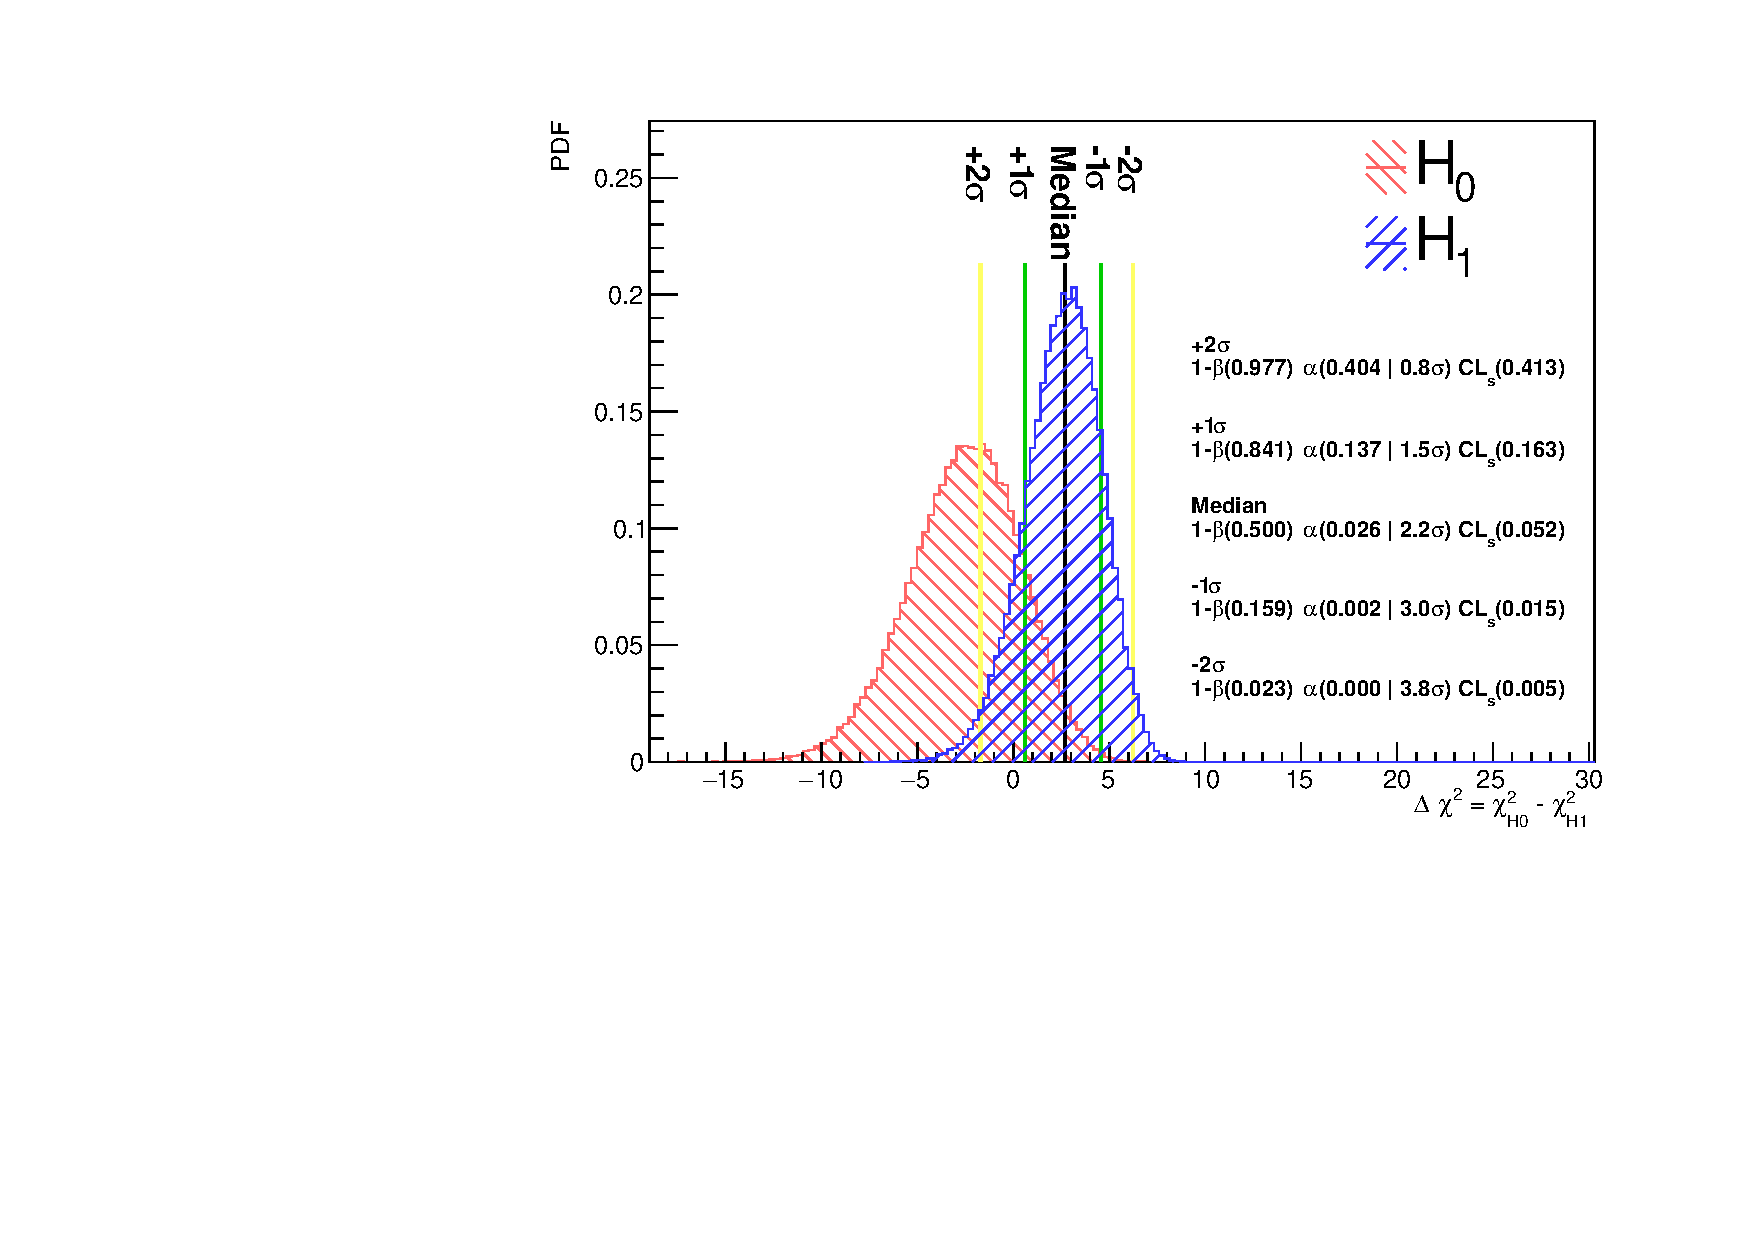
\includegraphics[width=1.00\textwidth]{Sensitivity/Exclusion/SBNfit_Cls_nue_1e0p_numu_reco_e_H1_newboxcut_noCCMEC_constrained_detsys.pdf}
    \label{fig:sensitivity_boxcut_const}
    \caption{Box Cut selection}
    \end{subfigure}
    \begin{subfigure}{0.45\textwidth}
    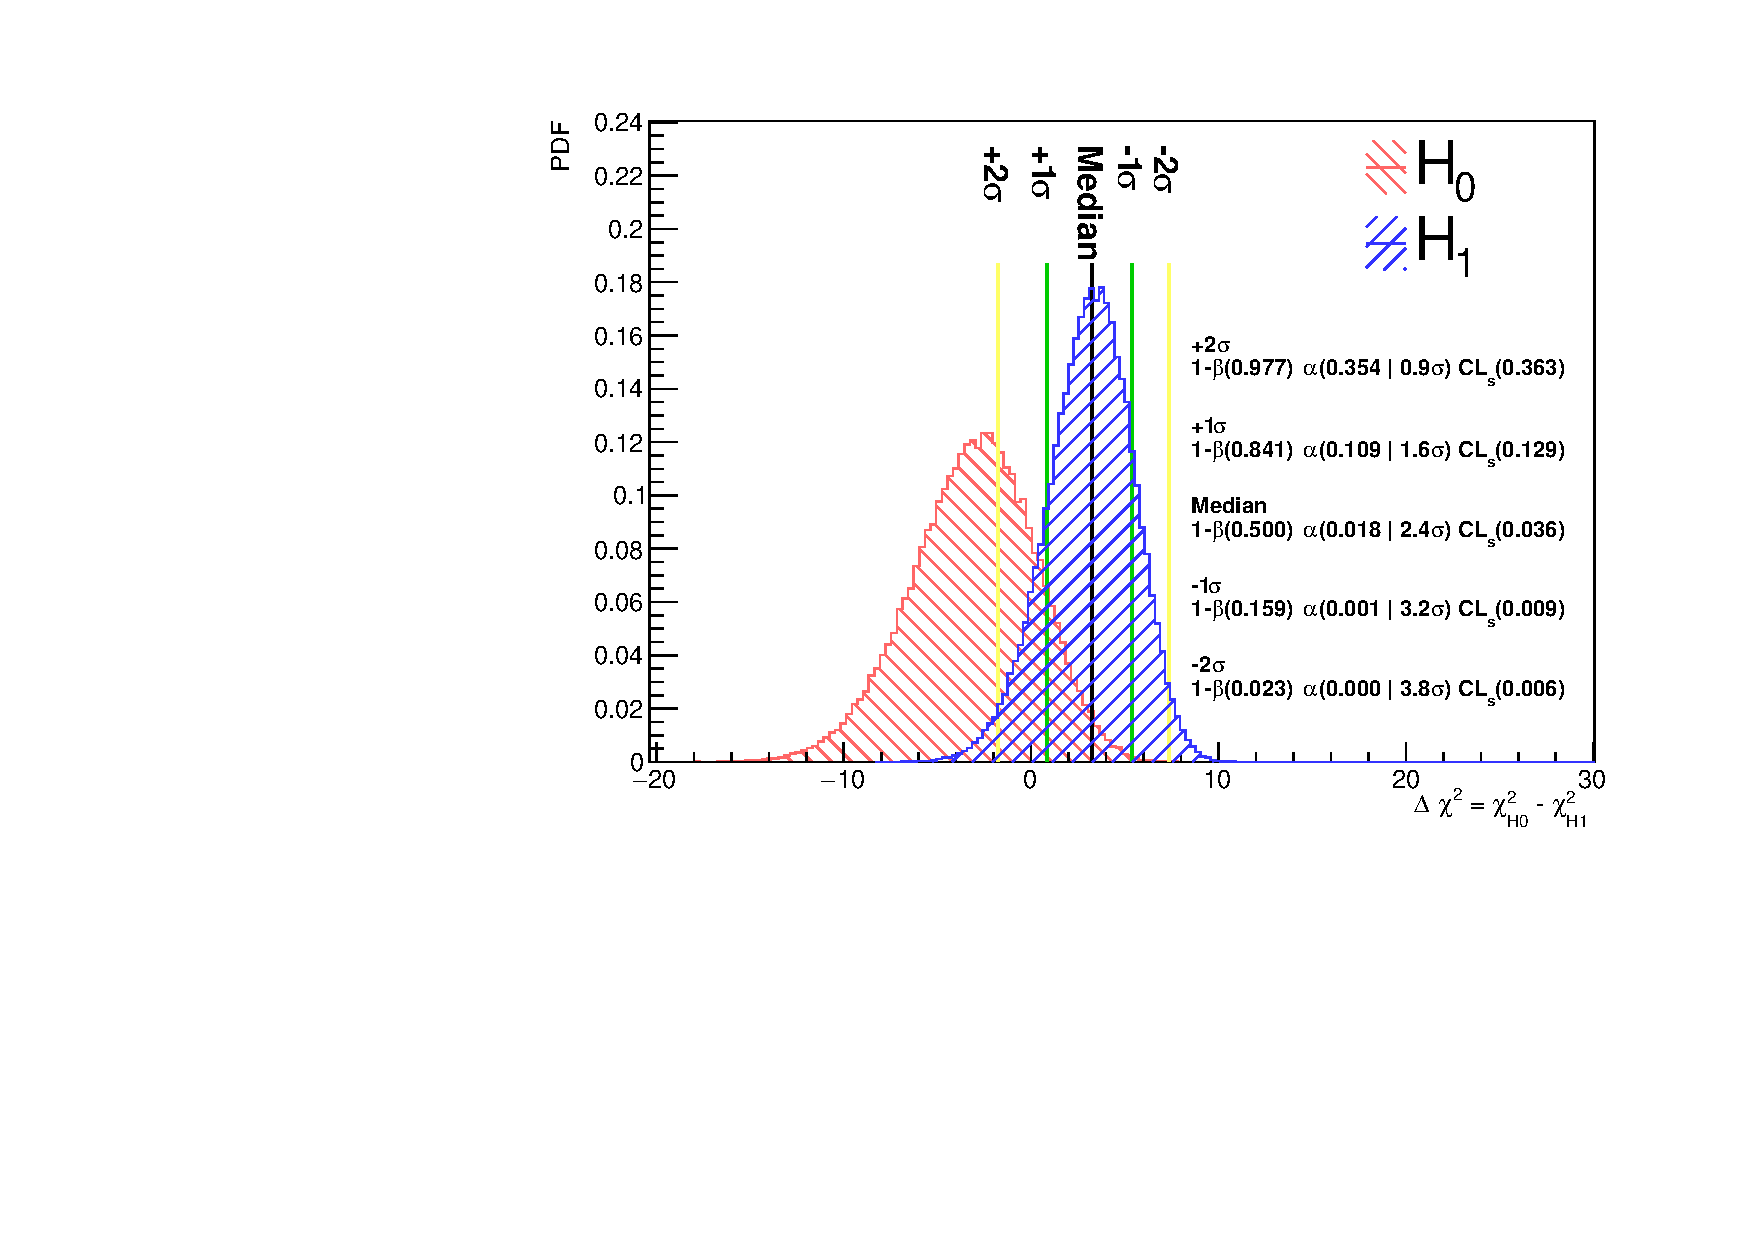
\includegraphics[width=1.00\textwidth]{Sensitivity/Exclusion/SBNfit_Cls_nue_1e0p_numu_reco_e_H1_newBDT_higheff_noCCMEC_constrained_detsys.pdf}
    \label{fig:sensitivity_bdt_loose_const}
    \caption{Loose BDT selection}
    \end{subfigure}
    \caption{Final exclusion sensitivity to the LEE unfolded signal of the \npsel selection with the \numu constraint. Sample is taken from combined Monte Carlo samples of Run 1, Run 2, and Run 3 and scaled to $6.95\times10^20$ POT.  (a) $H_0$ is the standard model and $H_1$ is the LEE model, (b) $H_0$ is the LEE model and $H_1$ is the standard model.}
    \end{center}
\end{figure}
\end{comment}{}
